\documentclass[conference]{IEEEtran}
\IEEEoverridecommandlockouts
% The preceding line is only needed to identify funding in the first footnote. If that is unneeded, please comment it out.
\usepackage{cite}
\usepackage{amsmath,amssymb,amsfonts}
\usepackage{algorithmic}
\usepackage{graphicx}
\usepackage{textcomp}
\usepackage{array}
\usepackage{enumitem}
\usepackage{xcolor}
\def\BibTeX{{\rm B\kern-.05em{\sc i\kern-.025em b}\kern-.08em
    T\kern-.1667em\lower.7ex\hbox{E}\kern-.125emX}}
\begin{document}

\title{SDPS: Blockchain Applied Student Data \linebreak Proof System \\
{\footnotesize \textsuperscript{*}WhaleShark}
}
\author{\IEEEauthorblockN{Su Min Kim}
\IEEEauthorblockA{\textit{Dept. Information Systems} \\
\textit{Hanyang University}\\
Seoul, Korea  \\
smjy9502@naver.com}
\and
\IEEEauthorblockN{Chul Woo Park }
\IEEEauthorblockA{\textit{Dept. Information Systems} \\
\textit{Hanyang University}\\
Seoul, Korea \\
tthoutan@gmail.com}
\and
\IEEEauthorblockN{Jae Yeon Shin}
\IEEEauthorblockA{\textit{Dept. Information Systems} \\
\textit{Hanyang University}\\
Seoul, Korea \\
 jaeyeon.shin.96@gmail.com}
\and
\IEEEauthorblockN{Jong Won Oh}
\IEEEauthorblockA{\textit{Dept. Information Systems} \\
\textit{Hanyang University}\\
Seoul, Korea \\
jongwon9978@gmail.com}
}
\maketitle

\begin{abstract}
 This document is about student data proof system based on Blockchain. Our group will make proof system that can minimize process of submitting and validating important documents like certificates, portfolios and research notes. By adopting Blockchain, it can assure 1) safe transaction while sending the documents, 2) reliability of documents and 3) simple process of checking documents. Our expectation to this software is to provide much comfortable way of sending documents which unnecessary process is discarded. \\
\end{abstract}

\begin{IEEEkeywords}
blockchain, private blockchain, hyperledger, software engineering, paperless, reliable transaction
\end{IEEEkeywords}

  \begin{table}[htbp]
  \renewcommand{\arraystretch}{1.7}
\caption{Role Assignments}
\begin{center}
\begin{tabular}{|p{1.5cm}|p{1.8cm}|p{4.2cm}|}
\hline
\textbf{Roles} & \textbf{{Name}}& \textbf{{Task description and etc.}} \\
\hline
User & Kim Su Min & User is person who actually uses the software. By using it, user gives feedbacks about the software and evaluate if the software is good or not. With this opinion, Developer keeps update the software's function and the quality of software. \\
\hline
Customer & Oh Jong Won & Customer is a person who requests for this software. It's job is to make requirements clear and to check if the software contains all options that is needed. After development of software is done, customer checks the software, compare between software and requirements and give feedback to developer to make software better.   \\
\hline
Software \linebreak Developer& Park Chul Woo & Software Developer's main job is to develop software based on customer's requirement. It's goal is to meet customer's need and make user feel comfortable while using this software.\\
\hline
\end{tabular}
\label{tab1}
\end{center}
\end{table}

  \begin{table}[htbp]
  \renewcommand{\arraystretch}{1.7}
\begin{center}
\begin{tabular}{|p{1.5cm}|p{1.8cm}|p{4.2cm}|}
\hline
\textbf{Roles} & \textbf{{Name}}& \textbf{{Task description and etc.}} \\
\hline
Development Manager & Shin Jae Yeon & Development Manager works as a bridge between developer and customer and user to make them to communicate well. It's job is to care both service side and development side. Also manager has to check if the requirements that customer has provided and design of software that developer is equal. \\
\hline
\end{tabular}
\end{center}
\end{table}

\vspace{5mm}

\section{Introduction}
When we have to submit some important documents such as certificates, portfolios or research notes, lots of process has to be done for single paper submission. First, we need to go to some place where we can print out our documents. Next, after printing out the documents, we have look for place to make scan of our document. After that, we have to send the image file to our mail system. Uploading the scan of document to submission destination, finally the process is done. 

What if this complex process could be done with just one click? The only thing we have to do is go into website, select what and where want to send and click submit buttons. This simple process can make us to save money as we don’t have to pay for printing out and scanning and can save time. To make this possible, we will develop SDPS which can submit important documents with simple process by using Blockchain technology. 

 A Blockchain is essentially a distributed database of records or public ledger of all transactions or
digital events that have been executed and shared among participating parties. Each transaction in the public ledger is verified by consensus of a majority of the participants in the system. And, once entered, information can never be erased. The Blockchain contains a certain and verifiable record of every single transaction ever made. Bitcoin, the decentralized peer­-to-­peer digital currency, is the most popular example that uses Blockchain technology. The digital currency bitcoin itself is highly controversial but the underlying Blockchain technology has worked flawlessly and found wide range of applications in various fields.

The advantages of Blockchain technology outweigh the regulatory issues and technical challenges. One key emerging use case of Blockchain technology involves “smart contracts”. Smart contracts are basically computer programs that can automatically execute the terms of a contract. When a pre-configured condition in a smart contract among participating entities is met then the parties involved in a contractual agreement can be automatically made payments as per the contract in a transparent manner.

We will going to upload documents that need to be certified into Blockchain ledger. If data is in ledger, we don’t need to suspect reliability of documents because it is hard to be modified. To be more specific, we will build a private Blockchain that only trustful participants such as school, companies and institute can join. If school uploads score certificates into ledger, nodes that are participating in private Blockchain can see the data that has been updated. 

By using this mechanism, we don’t need to worry about potential submission problem as data is propagated to nodes as soon as the data is uploaded. Also, the target place where receives the certificates such as companies or institutes, they do not have to double check the document’s reliability as data has no possibility of getting modified or counterfeited.

Service will be provided in website. We will use reactJS, HTML and CSS to build front part of web and NodeJS, MySQL and nginx for the back part. Nowadays, people care much about the design part of website. We will build a web which is clear, user-friendly and easy to use. There are separate pages for each participants and each has useful functions in it. 

For students, our software can guarantee more simpler process for submitting documents and sending with more secure way. Also, they can design their own first page of web, can make bookmarks for frequently using menus and can manage their own calendar to check for submission date. For schools and companies, they do not have to double check for the documents, can rely on data that has been submitted and can shorten the overall validating process. 

Further parts will discuss about requirements, related works, development environment and specification for our website.


\section{Requirements}
\subsection{Student}
This page is only for students who are in Hanyang University. In this page, students are be able to print or send certificates more easily. Also they can upload our portfolios or research note in here. As the main reason for students printing out their documents is for getting jobs. With calendar function, they can manage their deadline and see the process of submission.\\ 

\begin{enumerate}
	\item \textit {First Page (Log-in Page):} \\
    \begin{enumerate}
    	\item \textit {Log-in:} Log-in page is a first page that students can see when they enter to our website. They can use their HY-in ID and PW to log-in. By doing this, we don’t have to make another accounts.\\
        \item \textit {ID/PW search:} This page is for student who forgot their ID or PW. It is connect to HY-in system’s ID and PW search page.\\
    \end{enumerate}
    
    \item \textit {Main Page:} Main page appears when log-in is correctly done. Users can customize their own page and bookmark for the frequently using functions. \\
    \begin{enumerate}
    	\item \textit {Custom design:} Students are able to design their own page. They can select color and theme of the page. By providing variety of design, users can feel fun while they are using our website. Also, they can make the web that fits to each individual users’ needs.\\
        \item \textit {Main menu:} Our menu toolbar is different from the current design. We will going to place the toolbar in the middle of the page. It is consist of icons, so user can see more better and select the thing they want easily. \\
        \item \textit {Bookmark:} This function can make a shortcut to specific section. By implementing bookmarks, we can increase accessibility of website. It can minimize process that user has to go through.\\
    \end{enumerate}
    
    \item \textit {School Certificate page:} This page is to print or send the documents. We need to select the document that student wants to print and companies that student wants to send. Then the data is uploaded to the Blockchain ledger. Nodes can see the data as it is uploaded. This process can provide credibility of documents.\\
    \begin{enumerate}
    	\item \textit {Check \& Print:} This page is to see and print out the documents. It is needed in case the company that student wants to send document is not participating as node.\\
        \item \textit {Submit:} If company is participating in private Blockchain, user can use this page to submit their documents. Select the documents that they want to send and companies that they want to apply. Transaction works like this; If student press submit button, request will go to school. If school approve the request, the data will be send to company. \\
         \item \textit {Processing results:} User can check the request that they had made and the progress of it in this page. \\
    \end{enumerate}
    
       \item \textit {Portfolio management page:} We need this page to manage our portfolios. As portfolio contains lots of informations, it is hard to submit it one by one. This page can make portfolio automatically with given inserted data. \\
    \begin{enumerate}
    	\item  \textit {Extracurricular activity:} In this page, student should input the data such as name of activity, date, contents and certificates. \\
        \item \textit {Volunteer works:} In this page, student should input the data such as name of volunteer works, date, contents and certificates. \\
        \item \textit {Club activity:} In this page, student should input the data such as name of club, date and contents.\\
        \item \textit {License:} In this page, student should input the data such as certificate summary, date of acquisition, name of license and proof number. \\
        \item \textit {School activity:} In this page, student should input the data such as contents. of school activity.\\
        \item \textit {Internship:} In this page, student should input the data such as date of works, company name and contents of works.\\
        \item \textit {Check \& Submit:} User can check for portfolios in this page. They can select the data that they want to submit. Also they can print or download the whole portfolios. If submit button is pressed, request goes to school and send it to company if the request is approved.\\
        \item \textit {Processing results:} This page is to see the progress of request and the list of request that user has made.\\
    \end{enumerate}
    
       \item \textit {Research note:} We need this page to write a research note. Sometimes there are some dispute about the research patent and intellectual property. This page can make free from dispute. \\
    \begin{enumerate}
    	\item  \textit {Write:} In this page, student should input the data such as start date of research, research name, participants and contents of research.\\
        \item \textit {Check \& Submit:} User can check for portfolios in this page. They can select the data that they want to submit. Also they can print or download the whole portfolios. If submit button is pressed, request goes to school and send it to company if the request is approved.\\
        \item \textit {Processing results:} This page is to see the progress of request and the list of request that user has made.\\
    \end{enumerate}
    
       \item \textit {Schedule:} We need this page to check for job opening post and required documents. \\
    \begin{enumerate}
    	\item  \textit {Calendar:} By using calendar, user can see every job opening in one sight. \\
        \item \textit {My calendar \& Check List:} My calendar \& check list page shows the company that user made it as bookmark and progress of document submission. This page can provide student to manage their document easily and check for things that they have to do.  \\
    \end{enumerate}    
    
       \item \textit {My page:} My page is needed in case of changing theme or color of main page, revising personal information and checking for all requested records.\\
    \begin{enumerate}
    	\item  \textit {Personal Information:} Students can revise their personal information in this page. As SDPS is connected to HY-in, change will also be made in HY-in.\\
        \item \textit {Design:} Students can customize their own main page by changing color and theme. \\
        \item \textit {Total processing results:} Students can view all the records that they made and progress of requests.\\
    \end{enumerate}  
        
\end{enumerate}

\subsection{School}
School page is only allowed for school related faculties. School works as a middle administrator. They have authority to give approval to the requests that students made and give permission to the trusted companies to join in private Blockchain. So, most of details are focused on these two things.\\
\begin{enumerate}
	\item \textit {First Page (Log-in Page):} Log-in page is the first page that user sees. They have to type their ID and password to get into main page. As user of this page is also part of University, they do not need sign in process.\\
    \begin{enumerate}
    	\item \textit {Log-in:} School page have log-in page to get into main page. As school’s job is important in Blockchain, they should always be alert with information leak. So, if school faculty log-in to system, message will be send if log-in worked well or not.\\
    \end{enumerate}
    
    \item \textit {Main Page:} If user get into system correctly, they will see main page. Main page shows works that they have to do in order of importance. And it contains other options for managing Blockchain system.\\
    \begin{enumerate}
    	\item \textit {Work state:} We need this page to do works more efficiently. It shows request that they have to handle.\\
        \item \textit {Management menu:} It provides functions that user can use.\\
    \end{enumerate}
    
    \item \textit {Authentication:} We need this page to manage private Blockchain. It contains whether to give permission to company to enter into private Blockchain. Also this page can make approval to requests. \\
    \begin{enumerate}
    	\item \textit {Management of companies participating in the block chain:} This page is to handle companies’ requests for joining private Blockchain and control companies authorities.\\
        \item \textit {Approval of student requests:} This page is to handle student’s request of sending the documents to target destination.\\
        \begin{itemize}
	\item \textit {Sending information of the student:} We need this page to approve request of student’s information such as certificates of enrollment.\\
	\item \textit {Approval of portfolio information request:} We need this page to approve request of portfolio's contents.\\
	\item \textit {Writing portfolio information requested by student in block chain:} We need this page to approve request of portfolio to be sent to target destination.\\
	\item \textit {Writing research note data requested by student in block chain:} We need this page to approve request of research note to be sent to target destination.\\
	\end{itemize}
         \item \textit {Processing results:} This page summarizes the actions that user made. \\
    \end{enumerate}
    
       \item \textit {Blockchain management:} As school works as administrator of private Blockchain, this page is needed to manage Blockchain. Functions are mostly about checking the Blockchain environment.\\
    \begin{enumerate}
    	\item  \textit {Search participating companies:} This page is about checking reliability of the company. They look for abnormal transactions, cheating and etc..\\
        \item \textit {Check the status of the block chain:} This page is to do health-check in Blockchain network. This page can provide informations that is related to Blockchain quality.\\
    \end{enumerate}
        
\end{enumerate}

\subsection{Company}
This page is only made for company users. After they got permission to join in private Blockchain, they can get into main page. The main work for this page is to see the submitted documents.
\begin{enumerate}
	\item \textit {Registration page:} Different from student and school user, company needs to go through registration process. They need to provide trustful information to administrator which is school user. Also, they have to make ID and password in this page.\\
    
    \item \textit {First Page (Log-in Page):} This is the first page that user can see. If registration process worked successfully, they are able to use SDPS. \\
    \begin{enumerate}
    	\item \textit {Log-in:} They can type their ID and password to get into the main page.\\
        \item \textit {ID/PW search:} This function can provide user to find their missing ID and password.\\
    \end{enumerate}
    
    \item \textit {Main page:} After log-in worked well, user will get into main page. It briefly shows how many datas that they have received. \\
    \begin{enumerate}
    	\item \textit {Work state:} It shows total amount of data that they have received. By clicking it, they are able to look that information.\\
        \item \textit {Management menu:} It provides functions that user can use.\\
    \end{enumerate}
    
       \item \textit {Reading information page:} This page is for managing student’s data. Through this page, we can receive and browse documents. \\
    \begin{enumerate}
    	\item  \textit {Reading information:} Students’ informations are listed in tabular format. \\
        \item \textit {Print information:} This page is to make print of student’s documents.\\
    \end{enumerate}
        
\end{enumerate}

\section{Related Works}
We have researched for softwares that are doing similar works or having similar logics to ours. There are some tools that are providing similar service with different logics, in different platform or using overall Blockchain technology. By doing this research, we found out that Blockchain technology is widely used in various kinds of fields and it has a lot of potential powers. 

\subsection{Chain SIGN}
Chain SIGN is a first blockchain based contract platform made by blockchain platform specialized company 'TheRoof' and document management specialized company 'Cyberdime'. This is a new contract platform that assure trust by adding blockchain technology into original electronic contract system. It can have same effect with notarization in current electronic contract.

\subsection{EduCTX}
This platform is based on the concept of the EuropeanCredit Transfer and Accumulation System (ECTS). It constitutes a globally trusted, decentralized higher education credit, and grading system that can offer a globally unified viewpoint for students and higher education institutions (HEIs), as well as for other potential stakeholders, such as companies, institutions, and organizations. As a proof of concept, they present a prototype implementation of the environment, based on the open-source Ark Blockchain Platform. Based on a globally distributed peer-to-peer network, EduCTX will process, manage, and control ECTX tokens, which represent credits that students gain for completed courses, such as ECTS. HEIs are the peers of the blockchain network. The platform is a first step toward amore transparent and technologically advanced form of higher education systems. The EduCTX platform represents the basis of the EduCTX initiative, which anticipates that various HEIs would join forces in order to create a globally efficient, simplified, and ubiquitous environment in order to avoid language and administrative barriers

\subsection{New Blockchain Management System for Student Learning Data Developed by Sony}
Sony Corporation and Sony Global Education, a Sony subsidiary focused on global educational services, has developed a new platform for student education records based on Blockchain technology. The new solution will allow school administrators to consolidate and manage educational data for students in several schools, as well as record and refer to their learning history and digital transcripts with greater certainty. It will be developed with IBM Blockchain, and will use blockchain technology running on the IBM Cloud to track students’ learning progress, as well as to establish transparency and accountability of school achievement among students and schools. The platform will provide students with a digital and reliable record of their achievements that can be easily and quickly verified by any future employer or educational institutions. The data recorded on the platform is verified using IBM Blockchain and can be shared with stakeholders, including school administrators and prospective employers.

\subsection{MEDIBLOC}
MEDIBLOC is a project to solve current medical information system by using blockchain technology. It returns medical information that has been spread through each medical center. MEDIBLOC's goal is to create a world where individuals, medical providers, and medical researchers all enjoy a new medical experience by ensuring that medical information is securely distributed around individuals.

\subsection{CHAIN ID}
CHAIN ID issues a joint certificate through the consensus of the nodes (participants) in the network. The joint certificate is already authenticated through the consensus of the nodes and can be used freely throughout the network without any additional authentication. The smart contracts will guarantee the integrity of the data, ensuring that the certificate is trustworthy and without the risk of being altered. The information and status of the certificate is shared among the nodes in real-time so that all the participants will have the same information. By all the nodes having the same data, CHAIN ID can prevent single points of failure, such as hacking attempts that may happen in centralized network environments. Using CHAIN ID, users can experience a more convenient and reliable environment for making financial transactions.

\subsection{BankSign}
Customers who use Bank Sign can obtain a joint certificate from one bank, and they can easily use the mobile banking service of the other bank with simple authentication. The customer renewed the certificate every year when using the bank service and had to go through the registration and authentication process for each bank. However, Bank Sign makes it easy to access banking services from multiple banks at once. The authentication method has also been improved with convenience passwords, fingerprints, and patterns. The Bank Sign prevents the forgery of the certificate through the distributed agreement, which is a characteristic of the blockchain, and the synchronization of real-time authentication information between the banks. In addition to security, the block hain has increased security by encrypting communication segments and double-encrypting data and networks. This enhanced security has increased the validity period of the joint certificate from one year to three years.

\section{Development Environment}
\subsection{Choice of development platform}
\begin{enumerate} [font=\itshape]
  \item \textit{Platform used for developing: }
  \begin{figure}[htbp]
	\centerline{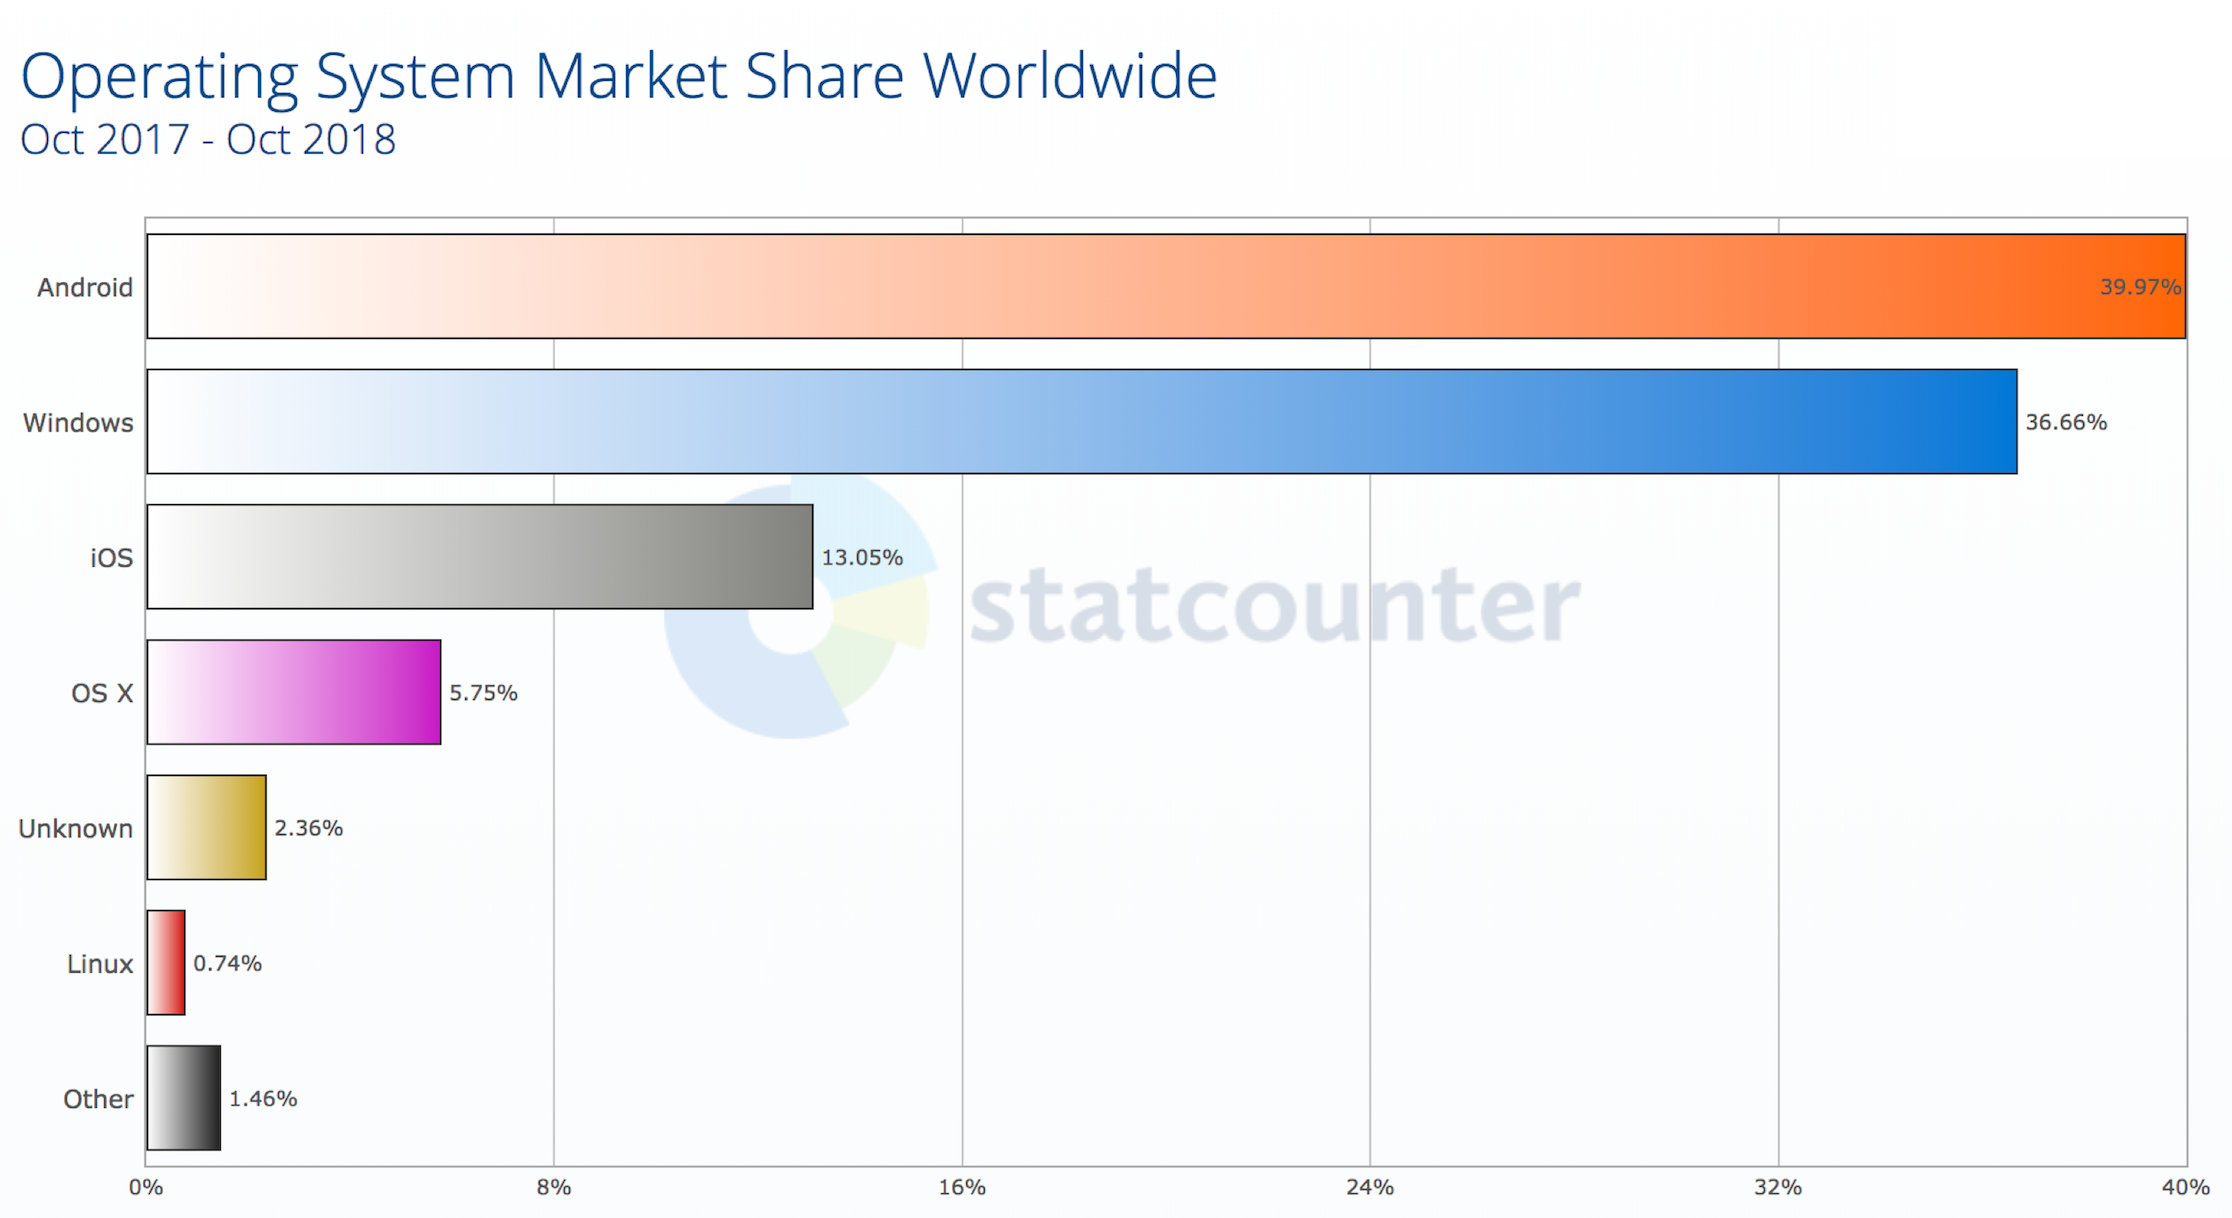
\includegraphics[width=89mm,scale=0.5]{graph.png}}
	\caption{Operating System Market Share Worldwide (2017.10 - 2018.10)}
	\label{fig}
	\end{figure}
	
  We will going to use Mac OS and Linux OS. Even thought Windows is still dominant in OS area, still Mac OS is a popular choice since lots of people prefer using Mac. We will not only use Mac OS but also we will use Linux by using Amazon Linux 2 AMI. Firstly, we will use AWS amazon linux 2 AMI free tier (t2.micro) to test environment of web applications. After that , we will use AWS amazon linux 2 AMI (t2.xlarge) to actually run web application. Docker will be used to test Blockchain's network. To build private Blockchain, we are going to use Hyperledger(Fabric) and Hyperledger composer(development tool).\\
  
   \item \textit{Programming language used for developing: }We are using various kinds of languages. For web frontend, we will use reactJS, HTML and CSS. For web backend, we will use NodeJS, MySQL and nginx. To make private Blockchain, we are going to use Go language. \\
   
    \begin{table}[htbp]
  \renewcommand{\arraystretch}{1.5}
\caption{Programming language used for developing}
\begin{center}
\begin{tabular}{|p{3cm}|p{4.7cm}|}
\hline
\textbf{Programming language} & \textbf{Reason} \\
\hline
HTML \& CSS & HTML is a markup language which is to compose basic web page. CSS adds design parts in web page. These two languages are popular choice of build website. \\
\hline
reactJS & react is one of javascript's library. It is used to make user interface. We will going to use this to do tasks that we want with simple action in GUI, not actually getting into Blockchain network directly. This can guarantee the usability of application. \\
\hline
 NodeJS &  This is one of library in server side javascript. This will act as a Web Application Server that handles user's dynamic request in web application environment. Also this will be used to interlock Blockchain application and Web applicaiton.\\
\hline
MySQL  & MySQL is open source DB which is using SQL language to add, view or modify data in database. It is used to store account information. \\
\hline
nginx & It is considered to be next generation server. This will be used to handle user's static processing directly. Static processing is sent to WAS. It provides reverse proxy function to hide information about WAS to user.  \\
\hline
Go language & Go is a programming language that Goole has invented. It is a compile language that has garbage collection function and provide parallelism. We will going to use this language to write chaincode which is smart contract in Hyperledger. \\
\hline
\end{tabular}
\label{tab1}
\end{center}
\end{table}

\vspace{50mm}
   
  \item \textit{Cost estimation (Software): } 
  \begin{table}[htbp]
  \renewcommand{\arraystretch}{1.5}
\caption{Cost estimation}
\begin{center}
\begin{tabular}{|p{3cm}|p{4.7cm}|}
\hline
\textbf{Software         } & \textbf{Task description        } \\
\hline
Github & Remote repository \\
\hline
Sublime text & Text editor \\
\hline
Mac OS X Mojave & Operating System \\
\hline
AWS amazon linux 2 AMI free tier (t2.micro) & Linux image that helps Amazon Web Services to be used in Amazon EC2 \\
\hline
AWS amazon linux 2 AMI (t2.xlarge) & Linux image that helps Amazon Web Services to be used in Amazon EC2  \\
\hline
 Mockflow & Wireframe tools \\
\hline
Hyperledger(Fabric) & blockchain framework implementation \\
\hline
Hyperledger composer(development tool) & Cooperation tool to accelerate development of smart contract \\
\hline
Docker & Opensource project to automate arrangement of Linux's application into software container \\
\hline
Total & 100,000\\
\hline
\end{tabular}
\label{tab1}
\end{center}
\end{table}
\end{enumerate}

\subsection{Software in use}
\begin{enumerate} [font=\itshape]
  \item \textit{Github: } It is a web-based hosting service for version control using Git. It is mostly used for computer code. It offers all of the distributed version control and source code management (SCM) functionality of Git as well as adding its own features. It provides access control and several collaboration features such as bug tracking, feature requests, task management, and wikis for every project.\\
   \item \textit{AWS amazon linux 2 AMI (t2.xlarge): } It forms a central part of Amazon.com's cloud-computing platform, Amazon Web Services (AWS), by allowing users to rent virtual computers on which to run their own computer applications. EC2 encourages scalable deployment of applications by providing a web service through which a user can boot an Amazon Machine Image (AMI) to configure a virtual machine, which Amazon calls an "instance", containing any software desired. A user can create, launch, and terminate server-instances as needed, paying by the second for active servers – hence the term "elastic". EC2 provides users with control over the geographical location of instances that allows for latency optimization and high levels of redundancy. \\
   \item \textit{DBMS: }It is the software that interacts with end users, applications, the database itself to capture and analyze the data and provides facilities to administer the database. The sum total of the database, the DBMS and the associated applications can be referred to as a "database system". Often the term "database" is also used to loosely refer to any of the DBMS, the database system or an application associated with the database.\\
   \item \textit{Sublime text: } It is a proprietary cross-platform source code editor with a Python application programming interface (API). It natively supports many programming languages and markup languages, and functions can be added by users with plugins, typically community-built and maintained under free-software licenses.\\
   \item \textit{IBM Hyperledger Fabric 1.0: }It is a blockchain framework implementation and one of the Hyperledger projects hosted by The Linux Foundation. Intended as a foundation for developing applications or solutions with a modular architecture, Hyperledger Fabric allows components, such as consensus and membership services, to be plug-and-play. Hyperledger Fabric leverages container technology to host smart contracts called “chaincode” that comprise the application logic of the system. Hyperledger Fabric was initially contributed by Digital Asset and IBM, as a result of the first hackathon.\\
   \item \textit{IBM Hyperledger composer(development tool): }It is a set of collaboration tools for building blockchain business networks that make it simple and fast for business owners and developers to create smart contracts and blockchain applications to solve business problems. Built with JavaScript, leveraging modern tools including node.js, npm, CLI and popular editors, Composer offers business-centric abstractions as well as sample apps with easy to test devops processes to create robust blockchain solutions that drive alignment across business requirements with technical development.\\
   \item \textit{Docker: }It is a computer program that performs operating-system-level virtualization, also known as "containerization". It was first released in 2013 and is developed by Docker, Inc. Docker is used to run software packages called "containers". Containers are isolated from each other and bundle their own tools, libraries and configuration files; they can communicate with each other through well-defined channels. All containers are run by a single operating system kernel and are thus more lightweight than virtual machines. Containers are created from "images" that specify their precise contents. Images are often created by combining and modifying standard images downloaded from public repositories.\\

\end{enumerate}

\subsection{Task distribution}
  \begin{table}[htbp]
  \renewcommand{\arraystretch}{1.7}
\caption{Task distribution}
\begin{center}
\begin{tabular}{|p{1.8cm}|p{6.1cm}|}
\hline
\textbf{Software} & \textbf{Task description} \\
\hline
Kim Su Min & Blockchain, Web Frontend\\
\hline
Park Chul Woo & Blockchain, Web Backend (DB)\\
\hline
Shin Jae Yeon& Web Frontend (React), Blockchain\\
\hline
Oh Jong Won  & Web Backend (Server,Network), Blockchain\\
\hline
\end{tabular}
\label{tab1}
\end{center}
\end{table}

\section{Specification}
\subsection{Student} 
‘Page For Student’ is the page which provides convenience for all papers students should get certified. To be specific, this page enables student’s grade, school register information, portfolio, and research note to be managed efficiently. Furthermore, all of those written contents could not only be evidenced, but also be sent safely with reliable.\\
\begin{enumerate}
	\item \textit {First Page (Log-in Page): }
	\begin{figure}[htbp]
	\centerline{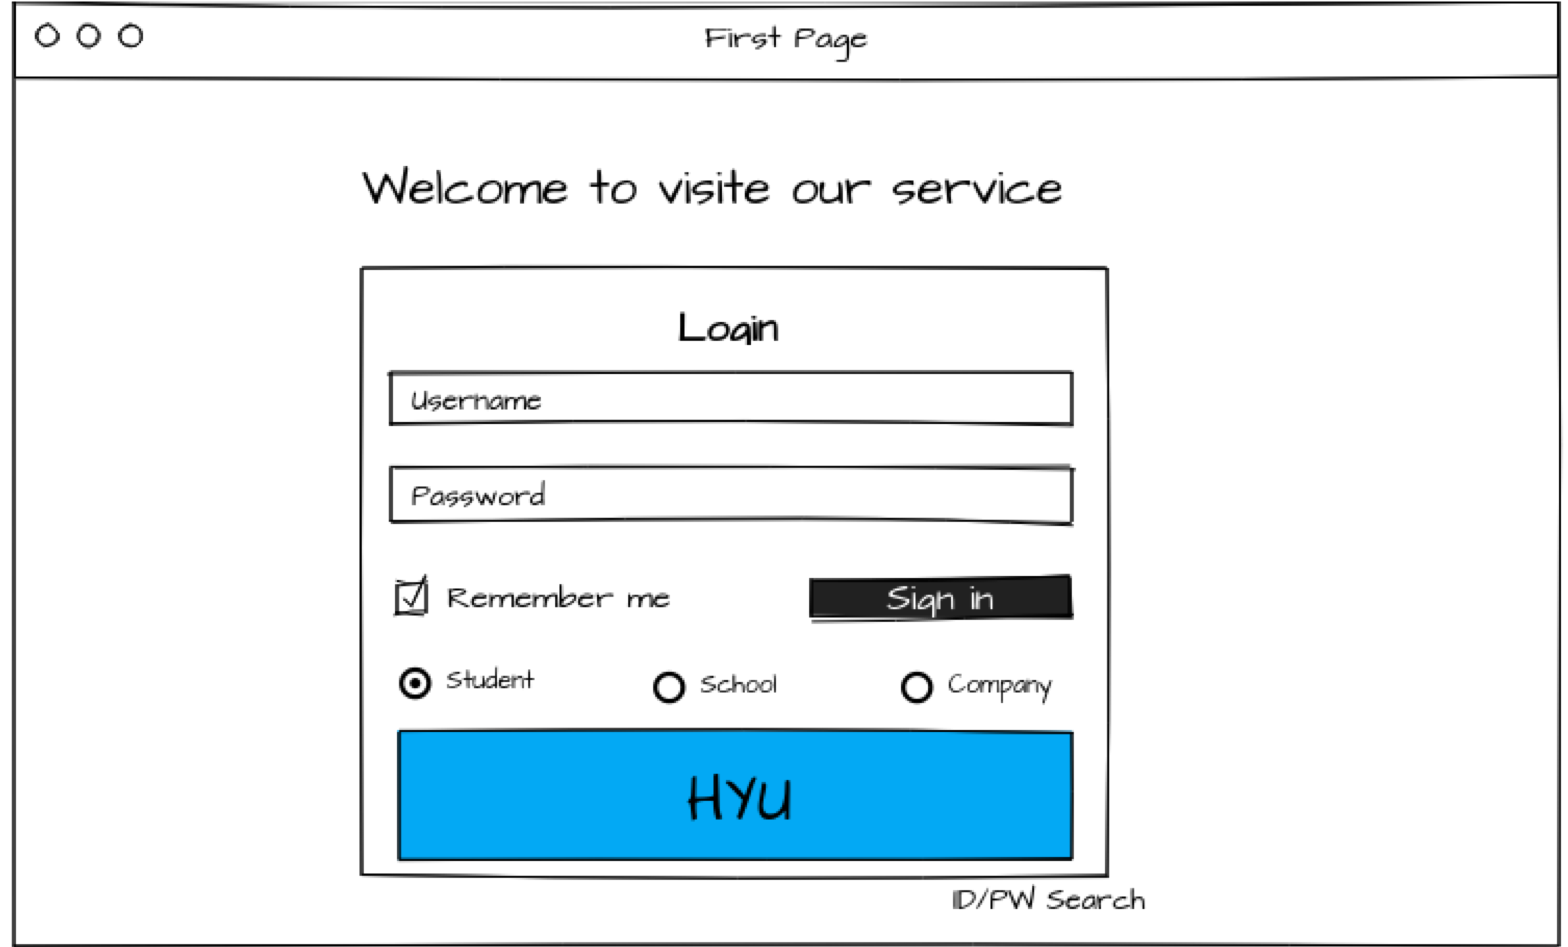
\includegraphics[width=89mm,scale=0.5]{student/login.png}}
	\caption{Log-in Page for SDPS}
	\label{fig}
	\end{figure}
	
	Users of our service must be registering in ‘Hanyang University Portal System(HY-IN)’ so that we do not offer any extra sign-up function. Instead, our system is trying to minimize the inconvenience of students and costs for maintenance of redundant data by enabling students to use their information from Portal in our system.\\
	
    \begin{enumerate}
    	\item \textit{Log-in: }Since member information from HY-IN is interconnected with our system, students can login without separate sign-up. So users firstly select ‘Student’ menu of three providing menus: Student, School, or Company. Secondly, HY-IN id and password are entered. Then, process of identification is followed so that students can move to main page if they success login. On the other hand, pop-up showing ‘Service is not available’ will be appeared and going back to login page again if inappropriate login information is entered more than three times.\\
        \item \textit{ID/PW search: }This page is for offering help to find the information if users lost their id or password. If users click the button shown, they can move to HY-IN’s ID and password recovering page. Users can find personal information by passing their own verification step using cell phone number or I-PIN.\\
    \end{enumerate}
    
    \item \textit {Main Page: }
    \begin{figure}[htbp]
	\centerline{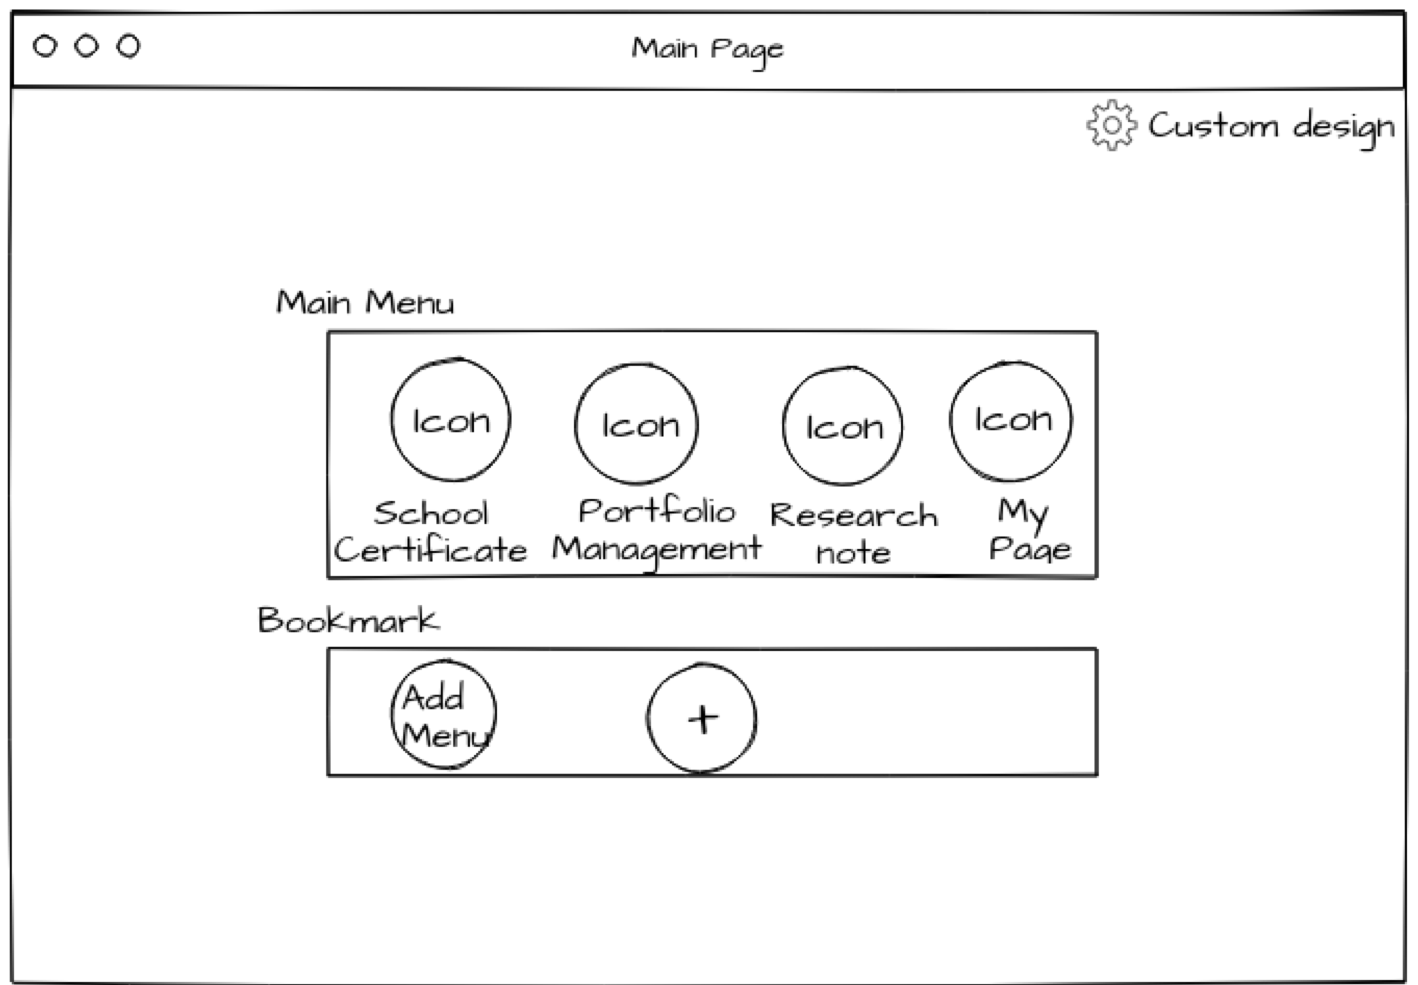
\includegraphics[width=89mm,scale=0.5]{student/mainpage.png}}
	\caption{Main Page for SDPS}
	\label{fig}
	\end{figure}
    
    Students can move on to this main page if they succeeded login. Images in screen are different separately depending on chosen design of individual students. \\
    \begin{enumerate}
    	\item \textit{Custom design:} If ‘custom design’ button on top of main page is clicked, this page will be shown. Users can choice their own preferable design in this page. For example, color and theme of main page can be diversified by users. Additionally, menus primarily used by students can be added to their own  ‘bookmark’. Those added menus are displayed on space for ‘bookmark’ in the main page. By applying this function, our system tries to provide specific UI(user interface) which is mainly focused on experience of users.\\
        \item \textit{Main menu:} Main menu of our system is shown intuitionally, staying away from existing stereotyped menus which listed by vertical and horizontal so that users can not only identify what function is in which page instinctively, but also choose requirable menu without hesitating. Each menu is consists of button and text. If users clicks button shown, they can move on to function shown. \\
        \item \textit{Bookmark:} Bookmark supports users by taking them to their mostly used functions. Added function from ‘Custom Design’ can be shown here and more functions can be supplemented according to user’s necessity by clicking ‘Add’ button on bookmark. With this Bookmark, we can minimize the unnecessary route via many other pages and maximize convenience of users. \\
    \end{enumerate}
    
    \item \textit {School Certificate page: }Previously, students cannot but request issue to school and submit that issued paper to relevant organization to hand in school issued documentation to institutions. Then, authentication of this submitted documentation should be checked by organization through school again. In this situation, the whole process becomes so cumbersome that waste of extra paper and loss of labor due to redundant work are caused. Our ‘School Certificate Page’ would fix that problem. In this page, if students choose the documentation they want to hand in, and organizations or companies(for those participated in private blockchain as nodes) they want to submit to, paper of student shown is uploaded to block. Then, that data is spread to other nodes. Since this written data of each node does not involve any risk of manipulation, omission and forging during transmission process, it can be used without any other verification process.\\
    \vspace{10mm}
    \begin{enumerate}
    	\item \textit{Check \& Print: }
	    \begin{figure}[htbp]
	\centerline{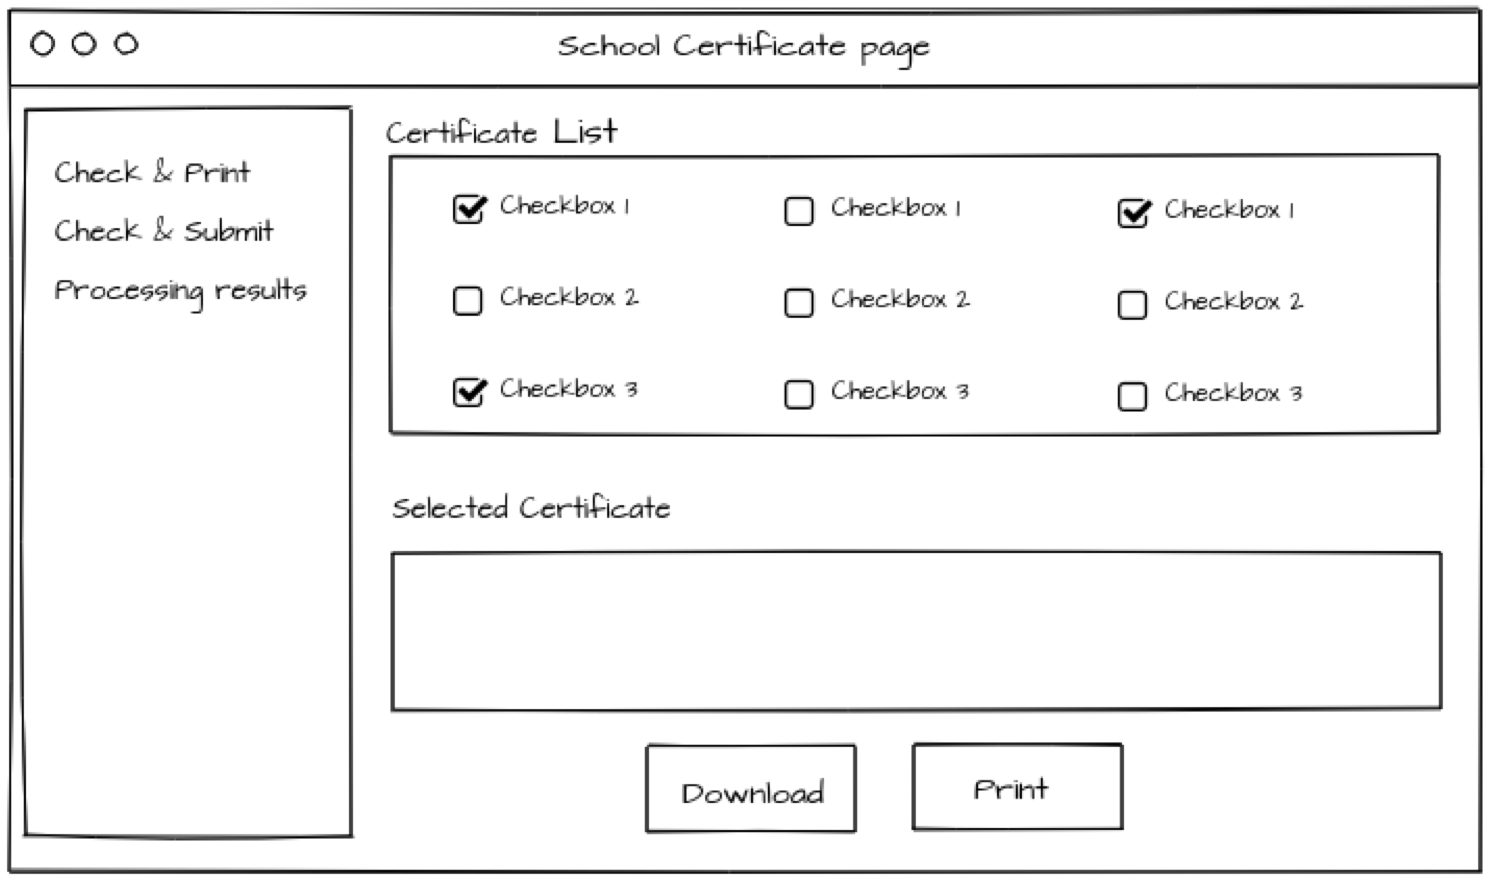
\includegraphics[width=89mm,scale=0.5]{student/certificate_check_and_print.png}}
	\caption{School Certificate Check \& Print Page for SDPS}
	\label{fig}
	\end{figure}
	
	In this page, users can inquire and print many different kinds of certificates from school. Especially, Check \& Print page can be utilized in specific following circumstances when students cannot use submit function of our system: scale of company and organization is not so large that they are not participated in private blockchain as nodes, or when submitting documentation for private purpose. This page is separated into two main parts which are section for making inquiry and the other for printing certification based on chosen data. \\
        \item \textit{Submit: }If places for submission are joined in private blockchain administered by the school, students can hand in certifications and papers issued by the school in Submit page. This page is consist of two main parts: section for selecting certificates, and the other for choosing companies or organizations students want to submit to. If all choices are made and ‘submit’ button is clicked, corresponding request is transmitted to school, and transaction is caused after approval of school took place. Through this transaction, certificates are sent to companies or organizations and transaction record shown is spread to other nodes. This process can be confirmed in ‘Processing result’ page or ‘Total Processing result’ page in ‘My page’. Since only private blockchain participated places are shown in the section for choosing place to submit, students could utilize ‘Check \& Print’ page to separately submit their certificates if there are no corresponding companies or organizations students want to submit in the list. \\
         \item \textit{Processing results:} 
         \begin{figure}[htbp]
	\centerline{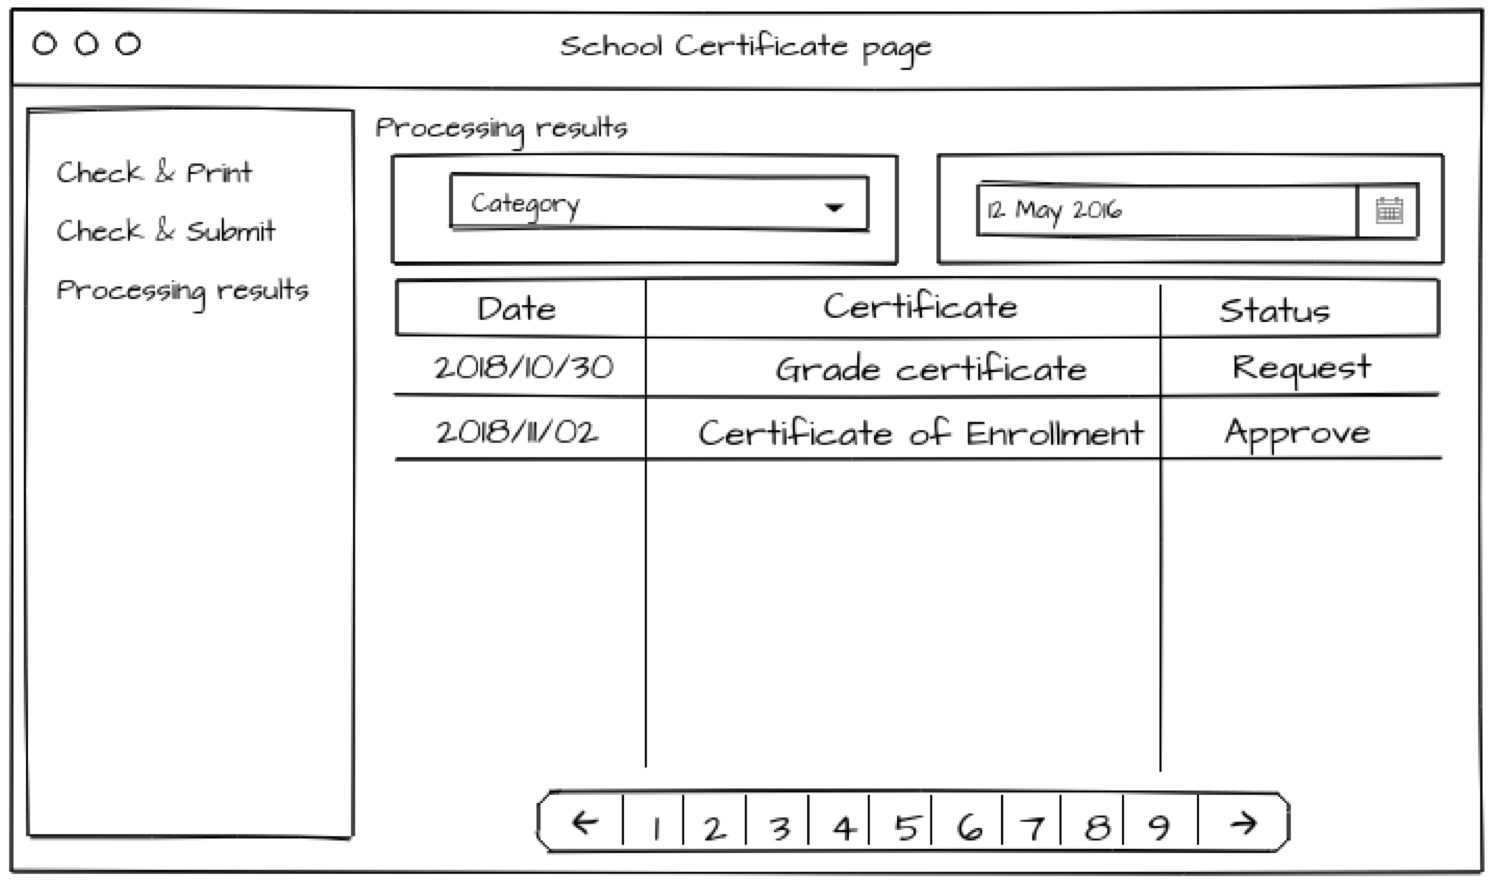
\includegraphics[width=89mm,scale=0.5]{student/certificate_processing.png}}
	\caption{School Certificate Processing results Page for SDPS}
	\label{fig}
	\end{figure}
         
         Record and progress of request can be identified in this page. Record part is categorized in specific kind and period. Inquiry of periodically categorized record includes monthly and weekly inquiry and period setting functions. With those functions, users can examine their request records in past and check for records and management process of inquiry corresponding to specific date. Besides,  progress has two main cases. The first case is process of ‘request, approval, complete sending’. Progress stays in ‘request’ phase when user requires transmission to specific facility. This phase moves on to ‘approval’ after school’s approval, and then ‘complete sending’ phase when the approval information causes transaction between school and facility. Transaction is commonly occurred when school clicks the approval button, however, ‘approval’ phase could be maintained if there are problems in blockchain or server of school. ‘Complete sending’ phase is shown only if the problems are solved. The second case is process of ‘request, rejection’. ‘Rejection’ phase occurs when student’s requested record makes errors, or there is difficulty to make transaction with participated company or organization as node so that submission is cannot be completed in a few days. \\
    \end{enumerate}
    
       \item \textit {Portfolio management page: }In recruiting, many companies demand portfolio to job seekers. Diverse information like A.4.a to A.4.h mentioned below is put in portfolio and inconvenient situation can be caused at this point since details like date and time of activity, history record and certificate should be submitted one by one. This page provides efficiently manageable service to solve the cumbersome problem by enabling users to manage many different kinds of data including date, context and paper of verification attached all together. If all of those uploaded information has appropriate form and content, school gives approval to those data. Based on this approval, student’s portfolio is proved primarily. Furthermore, the proved portfolio can be certified secondarily in the process of transmitting because blockchain is applied at here. Users can organize their portfolio with entered activities according to article and date. Under the premise of participation in private blockchain as node, the company can ask verification and submission of documentation to school. All process users should do is just clicking ‘submit’ button. However, if the company is not joining private blockchain as node, function of saving portfolio file as ‘pdf’ and printing it is provided by our system. Contents from A.4.a to A.4.f mentioned below is presented in each page with inquiry information entered until now. Page moves on to other page where users can enter new activities if ‘insert’ button at the bottom is clicked. Each page has function to inquire activities according to date and name which makes checking data of specific name, date and whether the school verified or not possible. Characteristic functions of A.4.a to A.4.f except for common things will be followed.\\
    \begin{enumerate}
    	\item  \textit{Extracurricular activity: }
	\begin{figure}[htbp]
	\centerline{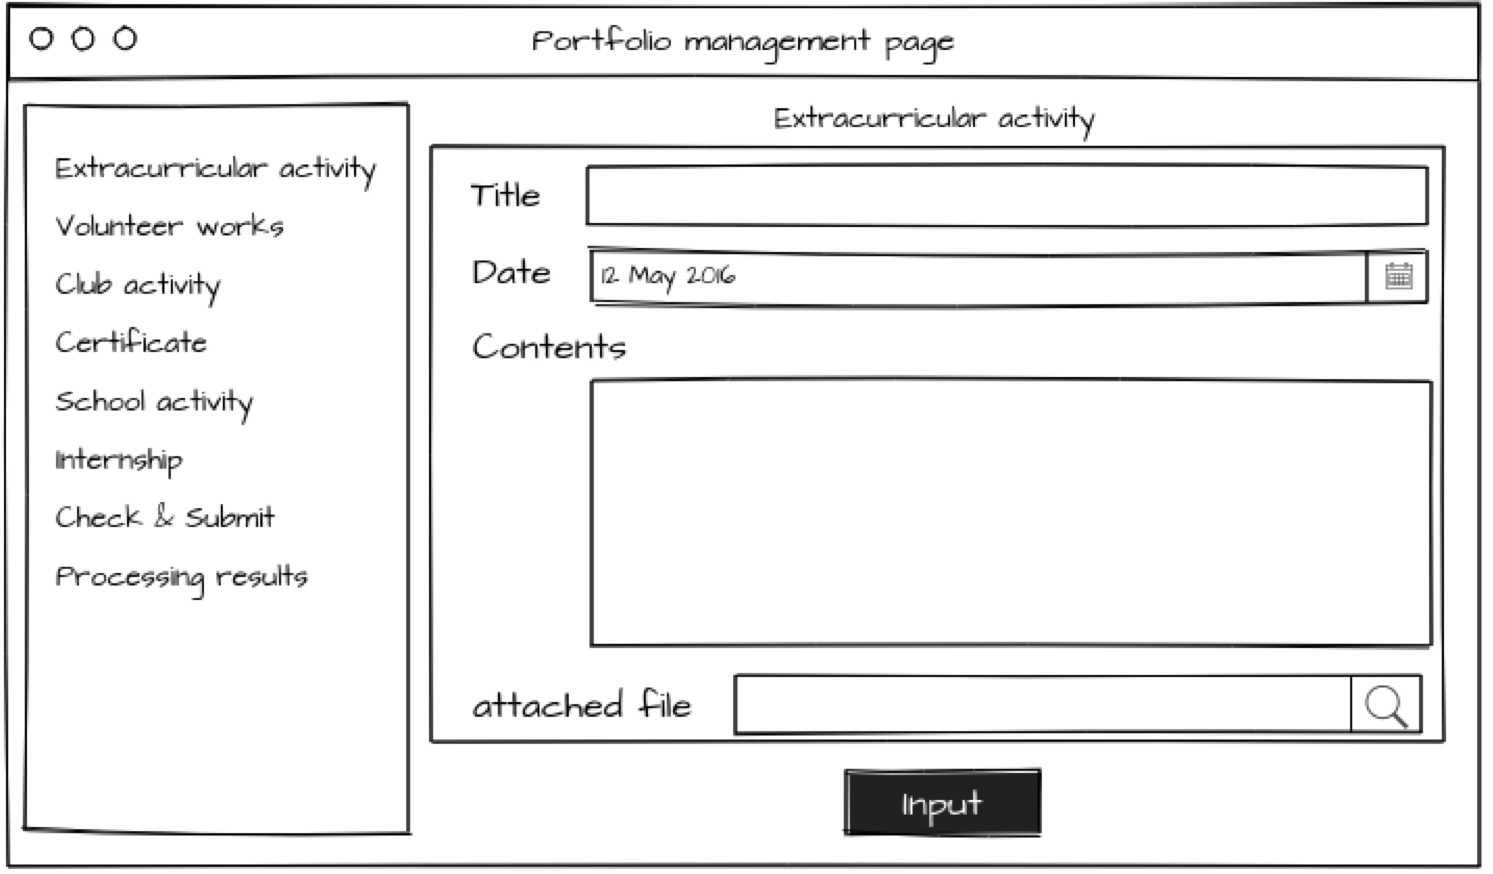
\includegraphics[width=89mm,scale=0.5]{student/portfolio_external_activity.png}}
	\caption{Portfolio Extracurricular activity Page for SDPS}
	\label{fig}
	\end{figure} 
	
	Students can input record of their extracurricular activities with name, date, content and certificate attached. School verify inserted record if inserted information is valid enough. Additional process of verification that might occur during submitting that activity record to companies could be simplified based on verification from school.\\
        \item \textit{Volunteer works:} Similar to extracurricular activity, students can enter record of the volunteer work with name, date, content and certificate attached. School confirms the work if enough information is inserted. Based on this confirm, extra unnecessary process of proof during submission to company could be avoided. Besides, users can also check their accumulated time of volunteer work.\\
        \item \textit{Club activity:} It is somewhat difficult to prove club activity since there is no specific paper for proof like certificate. In addition, there is no way to prove club activity if the club is broken apart. To deal with those kinds of problems, if students input name, date and content of the club, school certificates students’ club activity after checking club members and whether that club exists or not. Through this process, student’s club activity career can be verified. \\
        \item \textit{License:} There is difficulty for students to certificate each specific license when preparing for recruit since there are many different kinds of host institution issuing licenses and inquiry is possible only if acquisition date is clear. To handle this difficulty, school certificates the license information after confirming name, index, acquisition date and proof number of inquired licenses from students. Through this process, students can prove their record of licenses.\\
        \item \textit{School activity:} If company receives certification of school activity issued by that school and demands authentication of the specific activity to school again, paradoxical unnecessary process is caused. To solve the problem of that process, the school can input student’s school activity directly on the list shown and make verification without any extra certificates. With this process, students can demonstrate their own school activity as career.\\
        \item \textit{Internship:} In case of internship, it is difficult to prove career if certain amount of time is passed. Furthermore, students can go through confusion when inserting their exact work experience and details of work. To prevent this from happening, students can enter specific company they worked for, work period and details of business affairs on ‘Internship’ page. Then, school makes certification to inserted information so that students can prove their internship experience.\\
        \item \textit{Check \& Submit:}
        \begin{figure}[htbp]
	\centerline{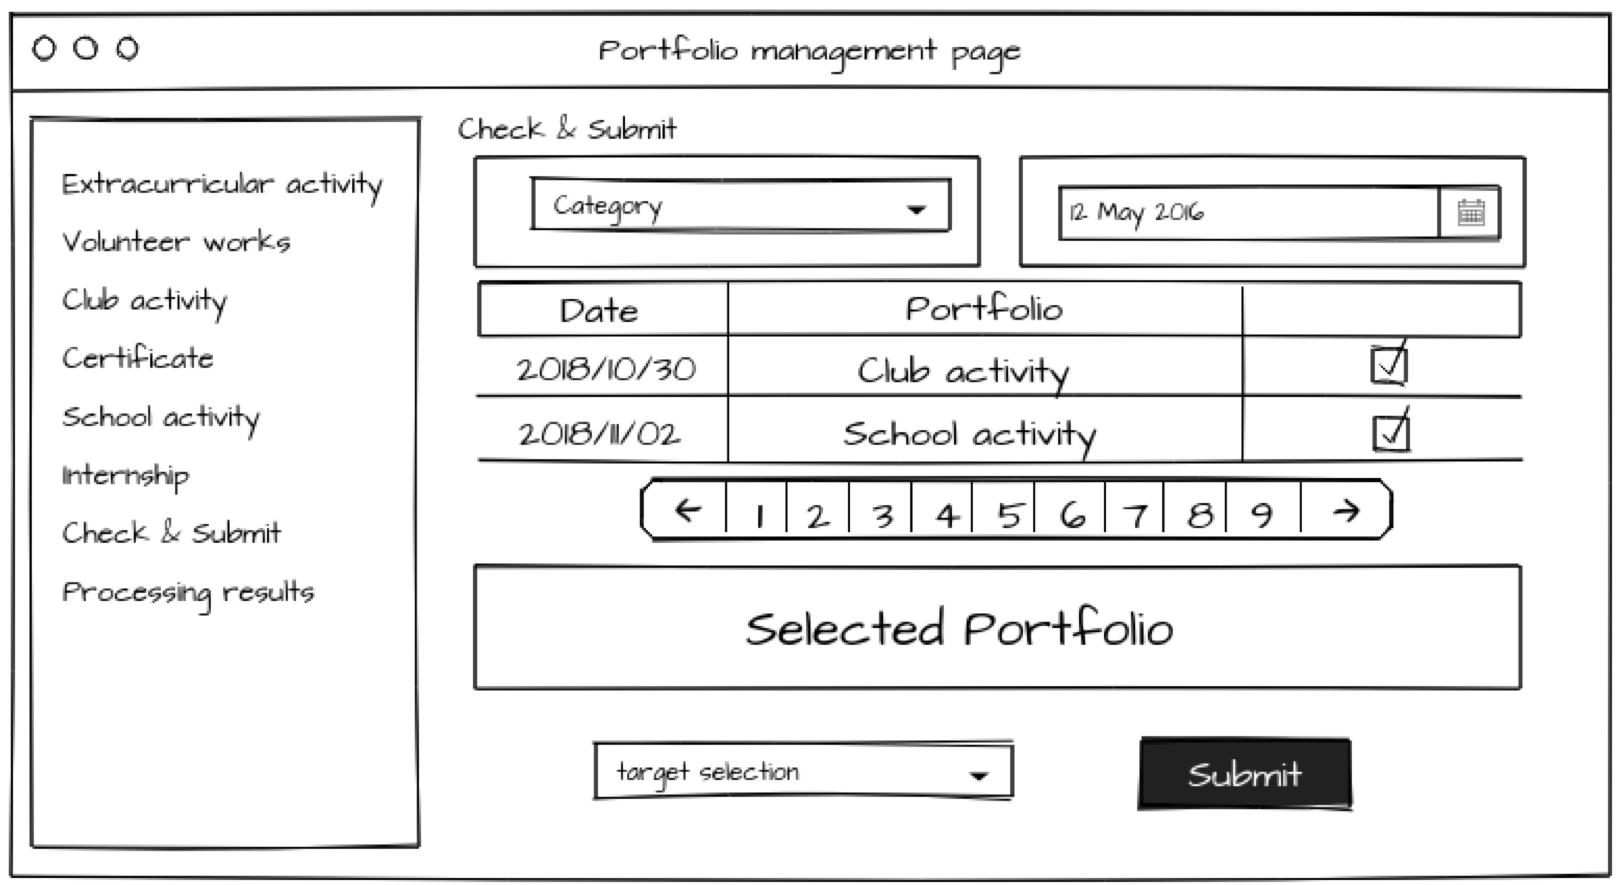
\includegraphics[width=89mm,scale=0.5]{student/portfolio_check_and_submit.png}}
	\caption{Portfolio Check \& Submit Page for SDPS}
	\label{fig}
	\end{figure}        
	
         If a place where students submit their information to is participated in private blockchain as node which is administered by school, student can submit portfolio through this page. This page is separated into three parts: section for choosing specific portfolio to submit, another for selecting company, the other for creating portfolio based on chosen items. Firstly, students can inquire their own portfolio at a single glance by sorting inserted data through setting according to date and type. Students can also choose what data should be in portfolio among inquired data. Secondly, If students pick places they hope to submit of the selection list and click the submit button, request shown is sent to the school. With school’s approval, student’s portfolio is submitted to company shown. Lastly, If there is no appropriate place on the list, students can click ‘creating portfolio’ button so that portfolio is made based on chosen items and can be printed or downloaded as pdf file.\\
        \item \textit{Processing results:} Users can recognize the record and progress of their request. In this page, only subjects which have finished requesting submission to company or organization can be inquired. Progress and detailed function are similar to A.c.3.\\
    \end{enumerate}
    
       \item \textit {Research note:} After inputting research date and contents, school loads those shown on the blockchain after receiving request for approval. By entering record which includes information about when the research was done and what subjects of research were, we are looking forward to protecting the research result in dispute regarding patent and copyright. Data on blockchain can be a great evidence which can demonstrate the achievement of research since it cannot be manipulated on blockchain.\\
    \begin{enumerate}
    	\item  \textit{Write:} This page is for writing research note. Date, research name, participants and contents can be entered with our system’s service which enables students to write diverse type of information including text, modification and photo. \\
        \item \textit{Check \& Submit:} This page is split into two parts: one for inquiring research note and the other for making request to school with inquired research note. Students can inquire their own portfolio at a single look by sorting inserted data through setting according to date and type. When student choose one specific research note among the lists, then they wait for school’s approval. After approval, research record shown is loaded on blockchain. At this point, it is very important for students to load their research note right after they finished it since the date of research data loaded is admitted as substantive date of the research note written.\\
        \item \textit{Processing results:} Users can realize what data they made request on and whole progress of request. Progress and detailed functions are same with A.3.c.\\
    \end{enumerate}
    
       \item \textit {Schedule: }Business recruitments and required documentations can be recognized in this page. Additionally, users can not only add specific companies to bookmark but also understand the progress of submitted paper instinctively with functions our system provides.\\
    \begin{enumerate}
    	\item  \textit{Calendar:} 
	\begin{figure}[htbp]
	\centerline{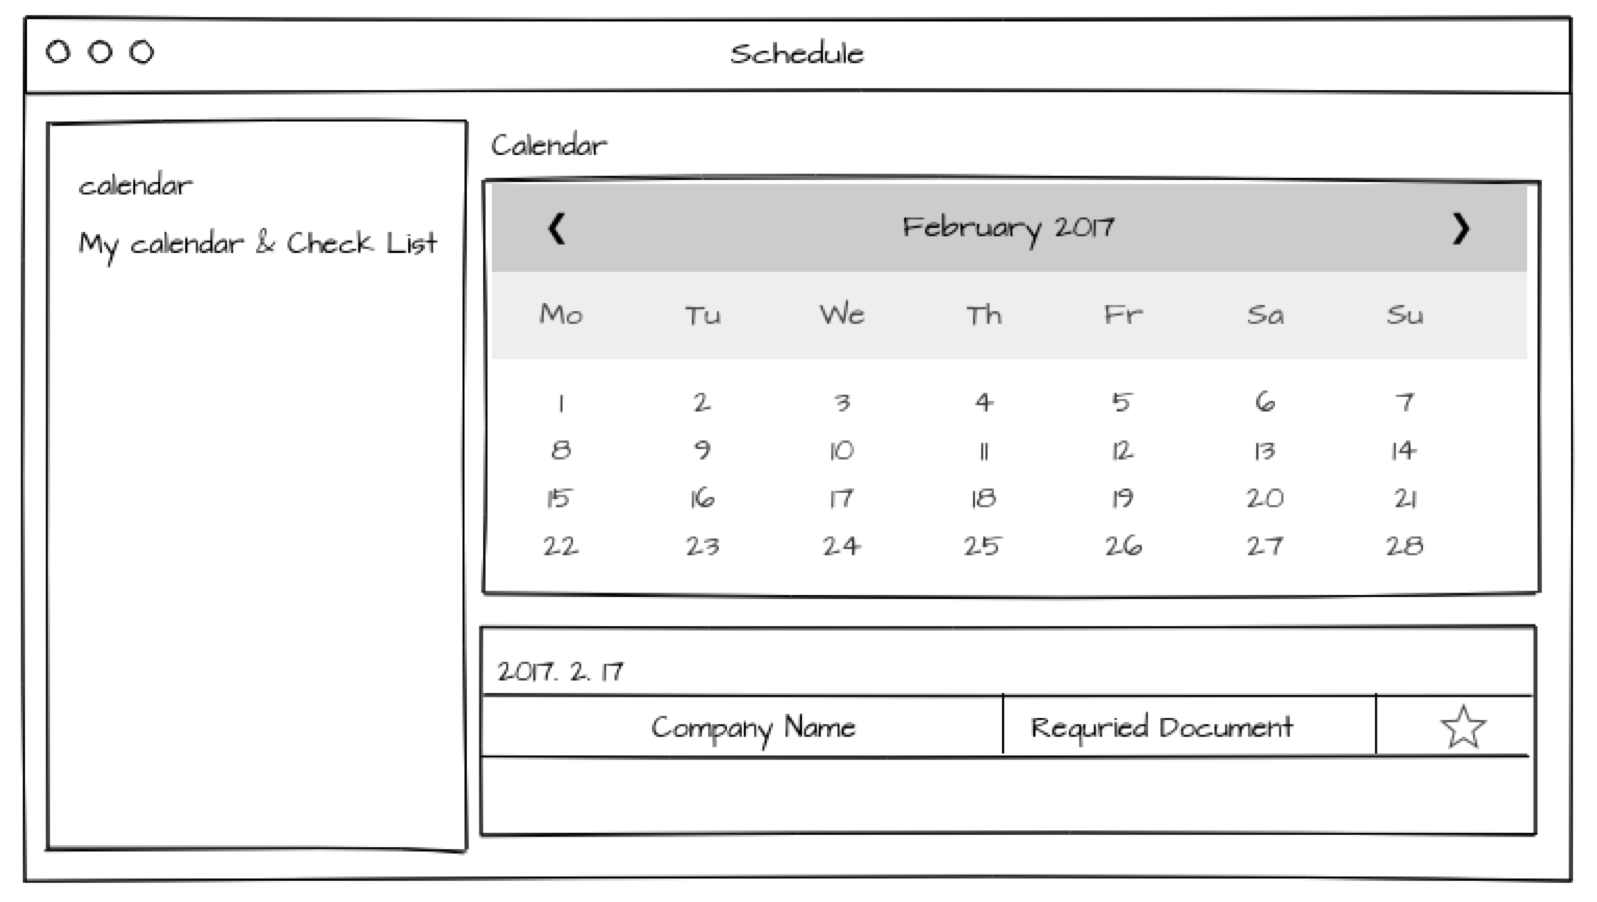
\includegraphics[width=89mm,scale=0.5]{student/calendar.png}}
	\caption{Schedule Calendar Page for SDPS}
	\label{fig}
	\end{figure} 
	
	This page is composed of two main parts: calendar typed table on the top and function of adding specific data they hope to on the bookmark. Information of each company’s recruitment can be checked from the table. As mentioned above, students can add companies they hope for on the bookmark and additional information is available in A.6.b page.\\
	\vspace{10mm}
	
        \item \textit{My calendar \& Check List:} 
        \begin{figure}[htbp]
	\centerline{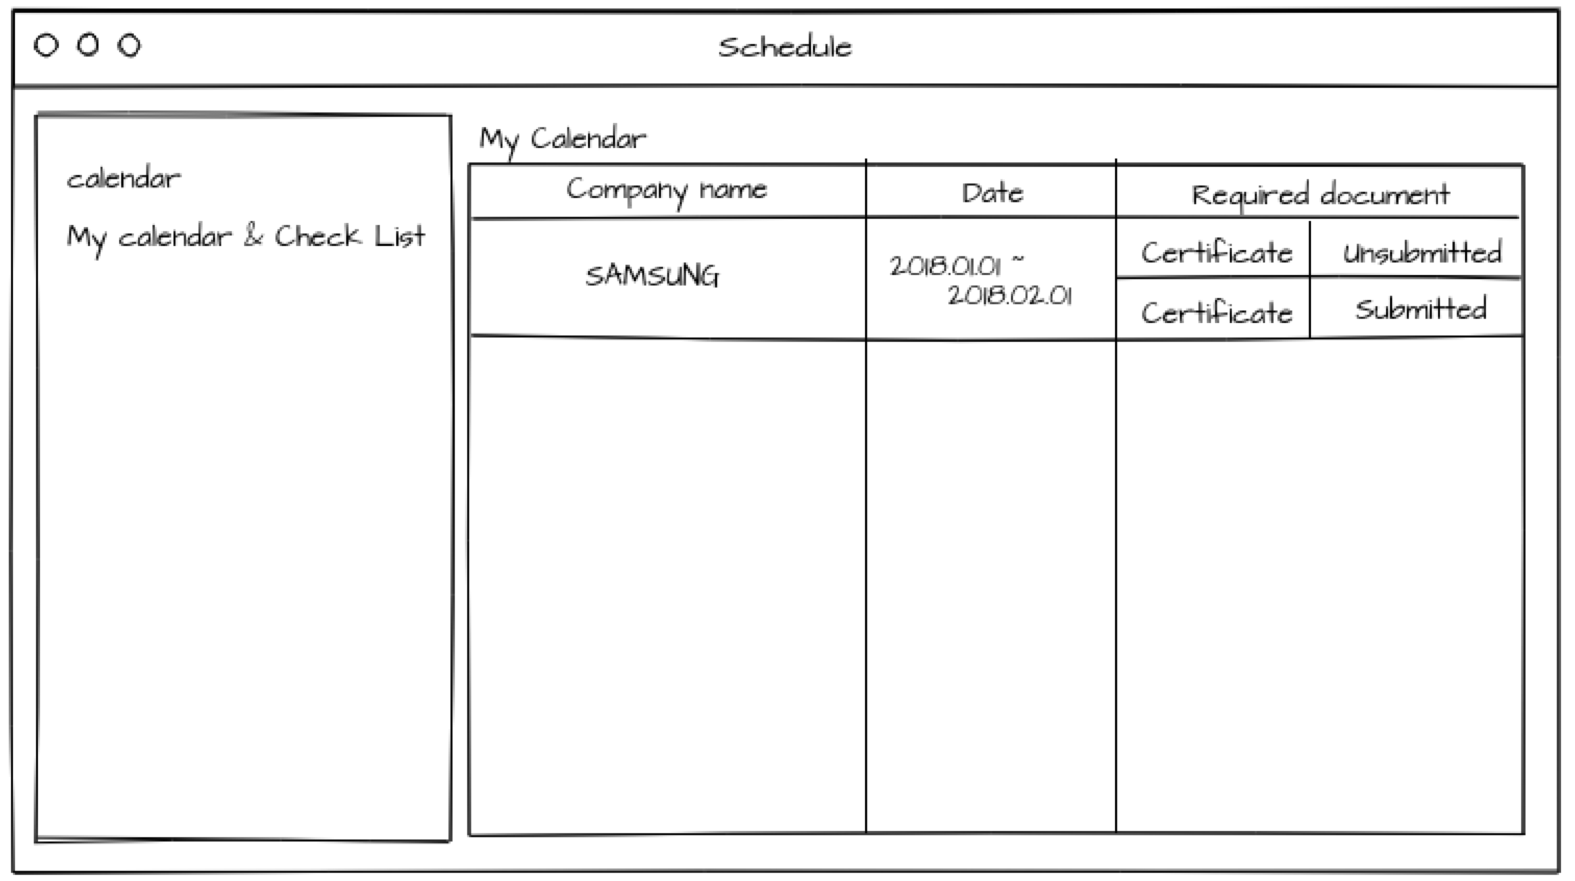
\includegraphics[width=89mm,scale=0.5]{student/My_calendar.png}}
	\caption{Schedule My calendar for SDPS}
	\label{fig}
	\end{figure} 
        
        This page marks information of each company’s recruitment added on the bookmark by students additionally. Each company’s recruitment information is like company name, recruitment date and required papers (grade, portfolio, etc.). From the perspective of required paper, specific sign will be shown according to the state of submission. For example, ‘submitted’ for submitted state, ‘unsubmitted’ for unsubmitted state and ‘approval’ for ongoing state so that students can simply recognize the list of companies they applied and progress at a single glance.\\
    \end{enumerate}    
    \vspace{30mm}
       \item \textit {My page: }
       \begin{figure}[htbp]
	\centerline{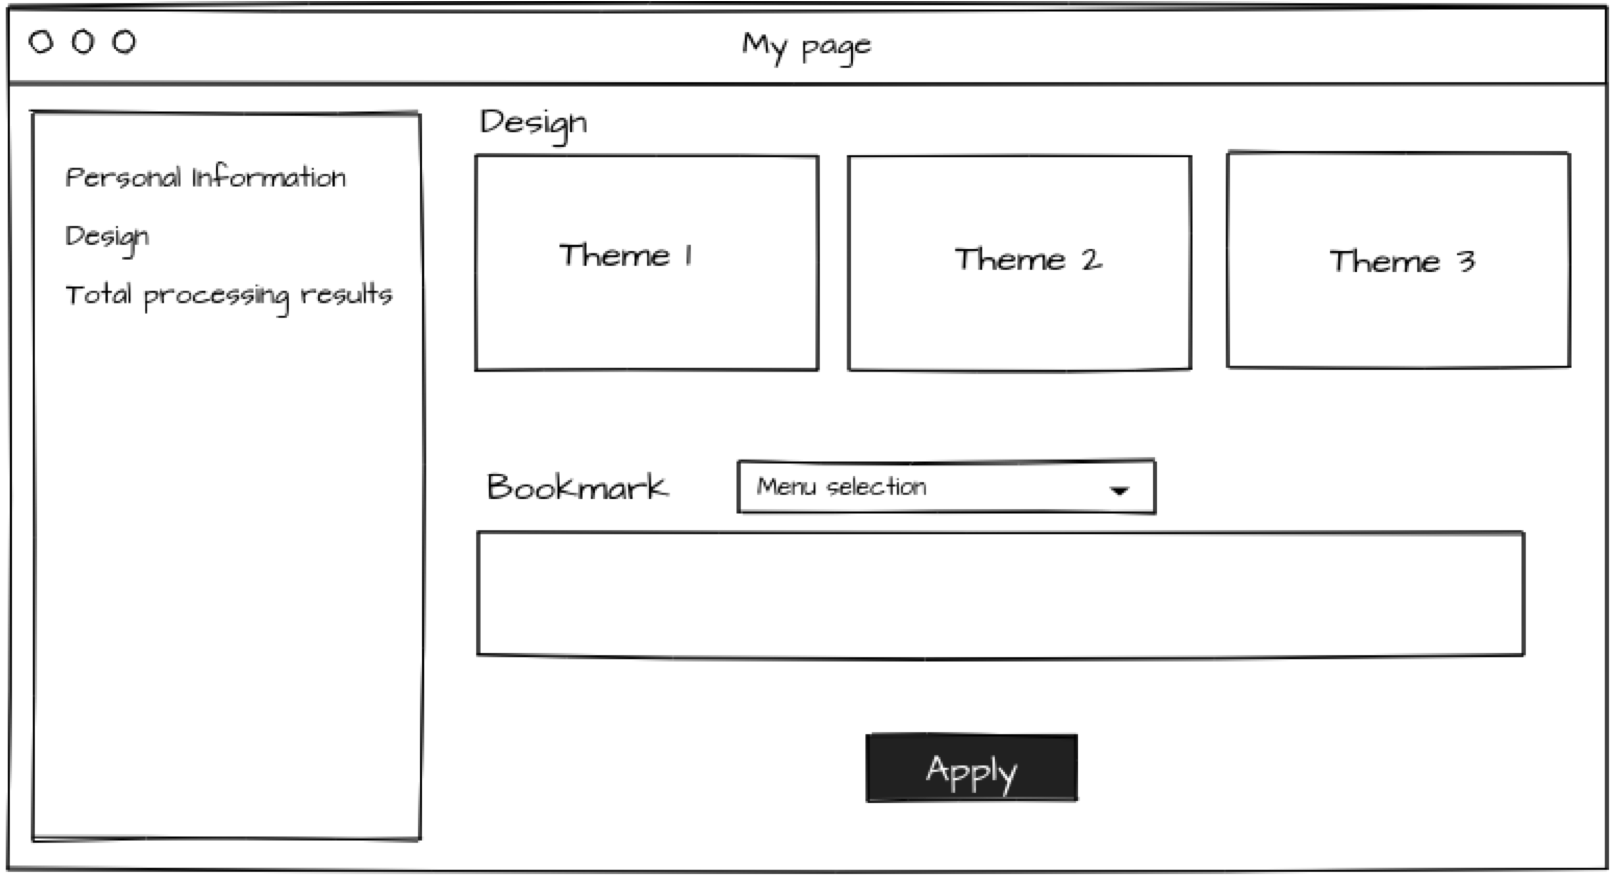
\includegraphics[width=89mm,scale=0.5]{student/Mypage_design.png}}
	\caption{My page page for SDPS}
	\label{fig}
	\end{figure} 
       
       This page primarily provides two functions. First of all, students can modify their personal information and color or theme of the main page. Secondly, progress of whole records requested by students is inquired and checked in this page.\\
    \begin{enumerate}
    	\item  \textit{Personal Information:} All information except for student’s name and distinct number given by school can be fixed. Modification of information made in this page is also applied in HY-IN’s member information. \\
        \item  \textit{Design:} This page is same with the page which can be seen by users if they click the ‘custom design’ button on top of main page. Detailed functions are same with A.2.a.\\
        \item \textit{Total processing results:} All records and progress of requests are grasped in this page. Records can be checked separately according to type (ex. portfolio, research note, certificate) and date. Progress and detailed functions are same with A.3.c.\\
    \end{enumerate}  
        
\end{enumerate}

\subsection{School}
School takes role of central executive of blockchain shown. Central executive decides whether approving participation or not when some users hope to participate in private blockchain as nodes. Additionally, some specific nodes can be modified or empowered in private blockchain. Role of central executive in relevant application is conducting data transmission request from students to specific companies. School which saves each of student’s individual information in the database administered by central executive can write and transmit the transmission record of blockchain’s sharing ledger from students who required data transmission to specific company. Also, in this transmission process, received certificate’s authentication is assured as data is received thanks to automatic proving program inherited in chain cord of smart contract. Through the conduction of central executive mentioned above, students can get rid of unnecessary process of printing paper documentation and submitting it to company themselves. Furthermore, company becomes convinced that received data is verified or not just by succeeding to receive without any extra checking processes.\\
\begin{enumerate}
	\item \textit {First Page (Log-in Page): }The central executive of the private blockchain is school which created and distributed the blockchain. School should make a choice whether using single centralized manager or many distributed managers. After that, the account decided as manager is logged in.\\
    \begin{enumerate}
    	\item \textit{Log-in:} The account decided as manager account can be logged in with id and password in manager login page. Manager is playing major role inside the blockchain so that leakage of manager information can cause severe danger to the blockchain. Therefore, special caution toward leakage is demanded. At this point, security of private blockchain is somewhat dependent to security of manager’s account. Our system has function to present success or failure alarm after trials of login are made based on that fact of security. \\
    \end{enumerate}
    
    \item \textit {Main Page: }
    \begin{figure}[htbp]
	\centerline{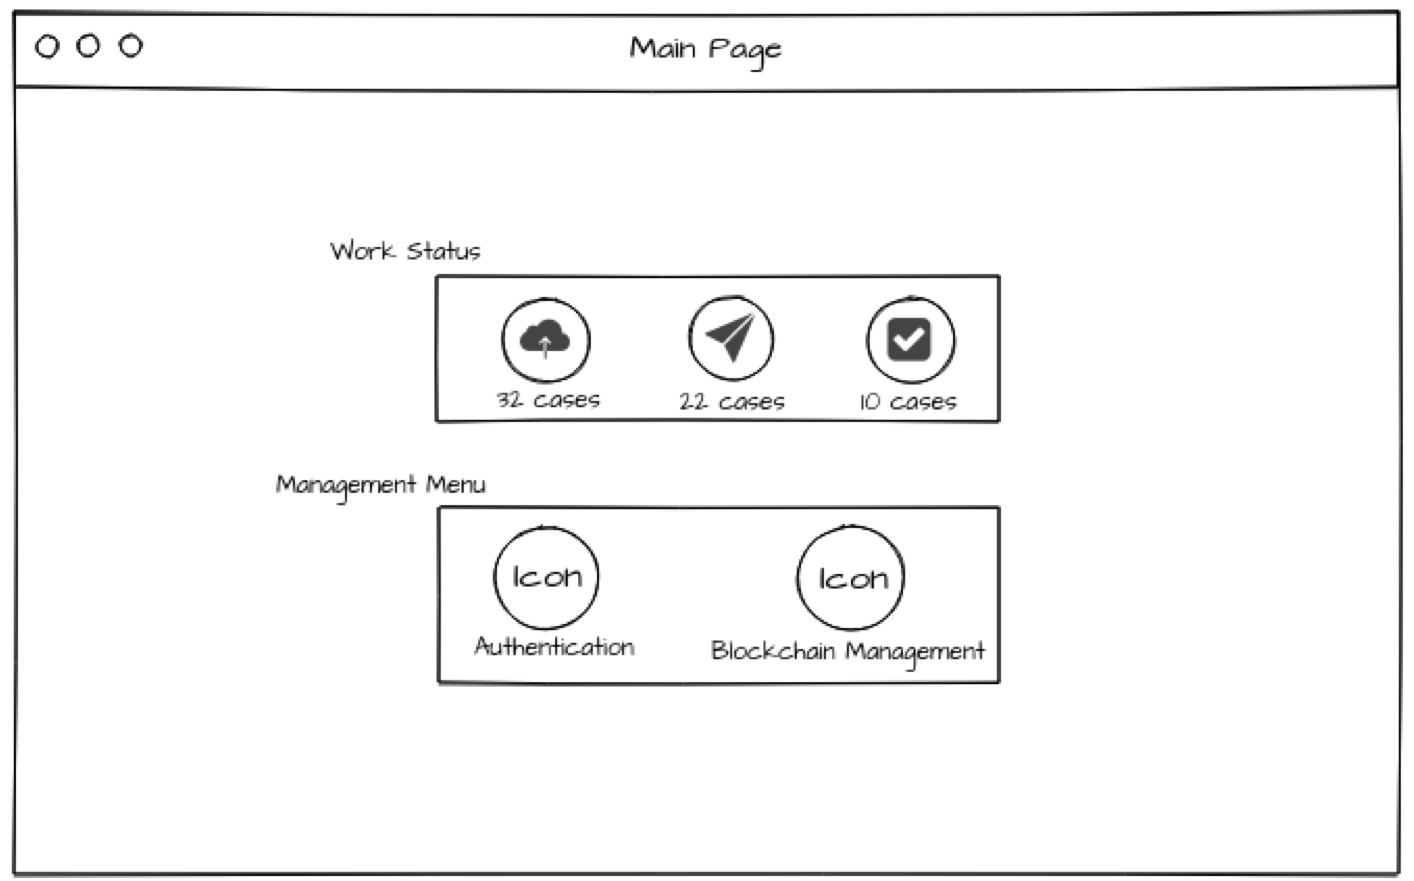
\includegraphics[width=89mm,scale=0.5]{school/mainPage.png}}
	\caption{Main page for SDPS}
	\label{fig}
	\end{figure} 
    
    This is the first page when users succeed login. Diverse menus including queue of important work what central executives should conduct in blockchain and menu for conducting many different kinds of functions directly are listed here.\\
    \begin{enumerate}
    	\item \textit{Work state:} This is central executive’s work conduction queue presented in main page. It is shown roughly and can also functions as anchor which allows user to move on to specific page if specific content is clicked. The total number of student’s requests waiting for approval and a few numbers of student’s requests which should be dealt with firstly (in order of greater past time is since requested) can be listed here. The requested time is also marked on the right side. With these contents, managers can identify how much time has been deferred for the approval of request and apply that information to decide whether offering approval right now or deferring additionally to the request.\\
        \item \textit{Management menu:} It provides navigation (function of anchor) for each function managers can conduct.\\
    \end{enumerate}
    
    \item \textit {Authentication}
    \begin{enumerate}
    	\item \textit{Management of companies participating in the block chain:} This page is for controlling chain participated companies’ authority and requests of companies which want to join in private block chain as nodes. Due to characteristics of private block chain, requests from companies which want to join in chain can be approved only after estimating whether the company is trustworthy or not. If some companies are estimated untrustworthy after getting approval, that approval can be canceled or that company’s authority can be removed inside of block chain.\\
        \item \textit{Approval of student requests:}
        \begin{figure}[htbp]
	\centerline{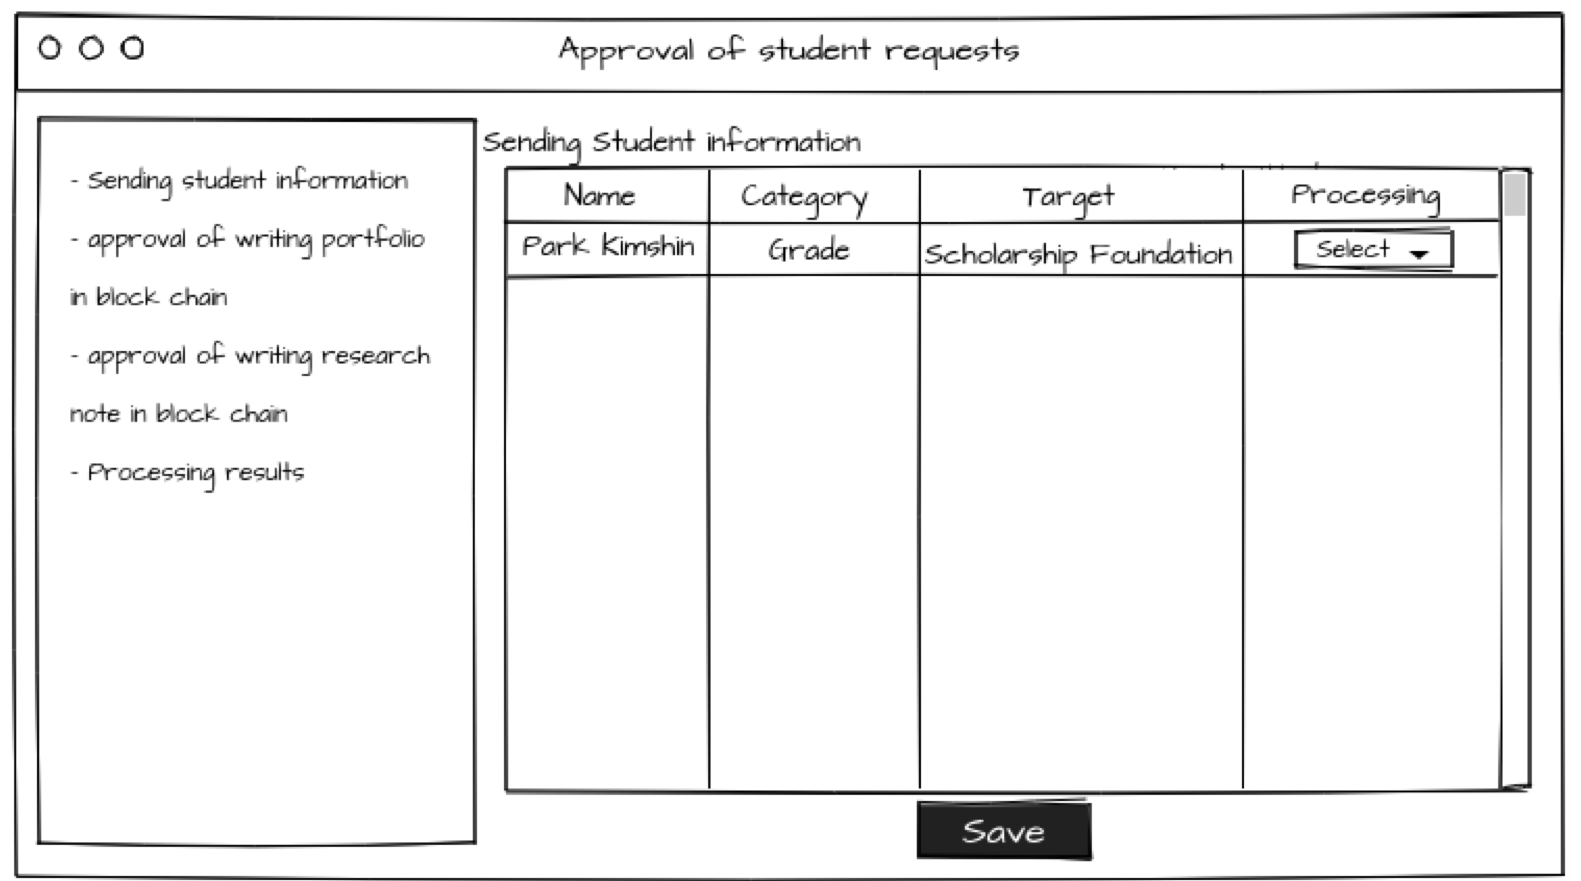
\includegraphics[width=89mm,scale=0.5]{school/approval_of_student_request.png}}
	\caption{Authentication Approval of student requests page for SDPS}
	\label{fig}
	\end{figure} 
        
        \begin{itemize}
	\item \textit{Sending information of the student:} If student makes request to specific company giving his or her information, the request is listed in authentication page of manager pages. Transaction is caused inside of block chain when central administrator clicks approval button and at this point, the information student hopes for transmitting is sent to specific company through block chain. The data of transaction is recorded inside of block chain’s sharing ledger.\\
	\item \textit{Approval of portfolio information request:} If students enter their portfolio through page for student with contents in form and enough proof materials and then make request to central manager for approval, the school verifies the activity. On the other hand, if contents are not in form and not enough proof materials were attached, the school can take action of ‘rejection’.\\
	\item \textit{Writing portfolio information requested by student in block chain:} If student makes request to specific company giving his or her portfolio, the request is listed in authentication page of manager pages. Transaction is caused inside of block chain when central administrator clicks approval button and at this point, the information student hopes for transmitting is sent to specific company through block chain. The data of transaction is recorded inside of block chain’s sharing ledger.\\
	\item \textit{Writing research note data requested by student in block chain:} Students can secure reliability and clarity of research note by recording it in block chain. Those students’ requests are listed in manager page and central execute write content and written date of the research note in sharing ledger of block chain after checking information in case of need. This function can offer dependability and transparency of research note’s authentication and written date information.\\
	\end{itemize}
         \item \textit{Processing results:} 
         \begin{figure}[htbp]
	\centerline{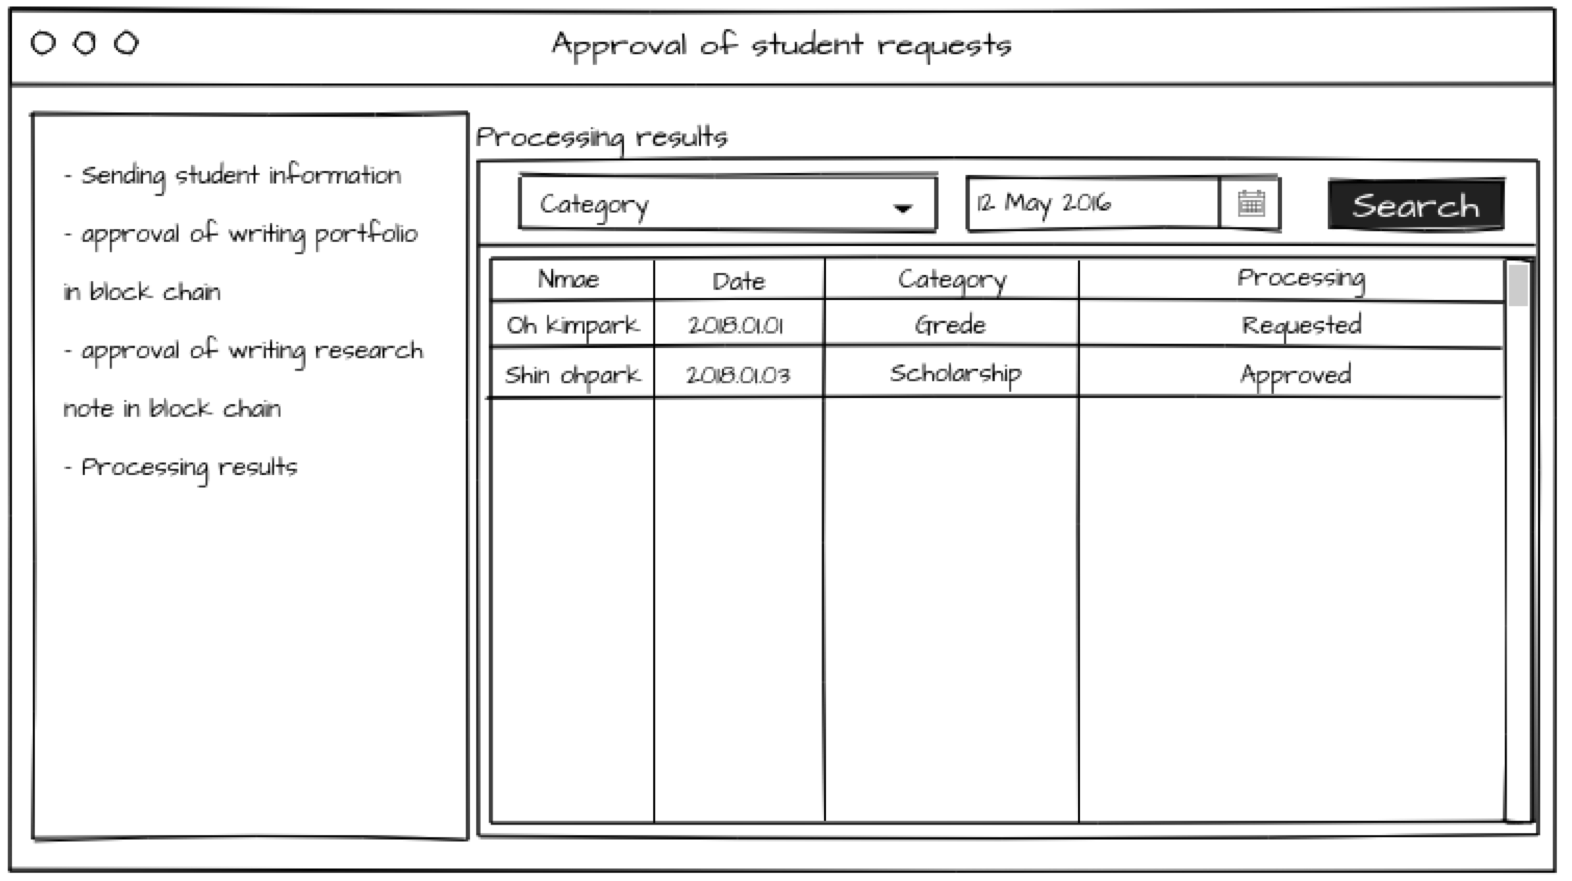
\includegraphics[width=89mm,scale=0.5]{school/processingResult.png}}
	\caption{Authentication processing results page for SDPS}
	\label{fig}
	\end{figure} 
         
         When administrator clicks submit button after students’ many different kinds of requests, appropriate transactions for each request is conducted and the processing result is returned to page. If there were some errors during transaction process, the result is presented as ‘rejection’, while ‘submit completed’ sign occurred for submission request and ‘record completed’ regarding portfolio and research note. And in case of submit button clicked by manager but result value not returned yet in block chain, ‘approval’ sign is presented.\\
    \end{enumerate}
    
       \item \textit {Blockchain management}
    \begin{enumerate}
    	\item  \textit{Search participating companies:} 
	\begin{figure}[htbp]
	\centerline{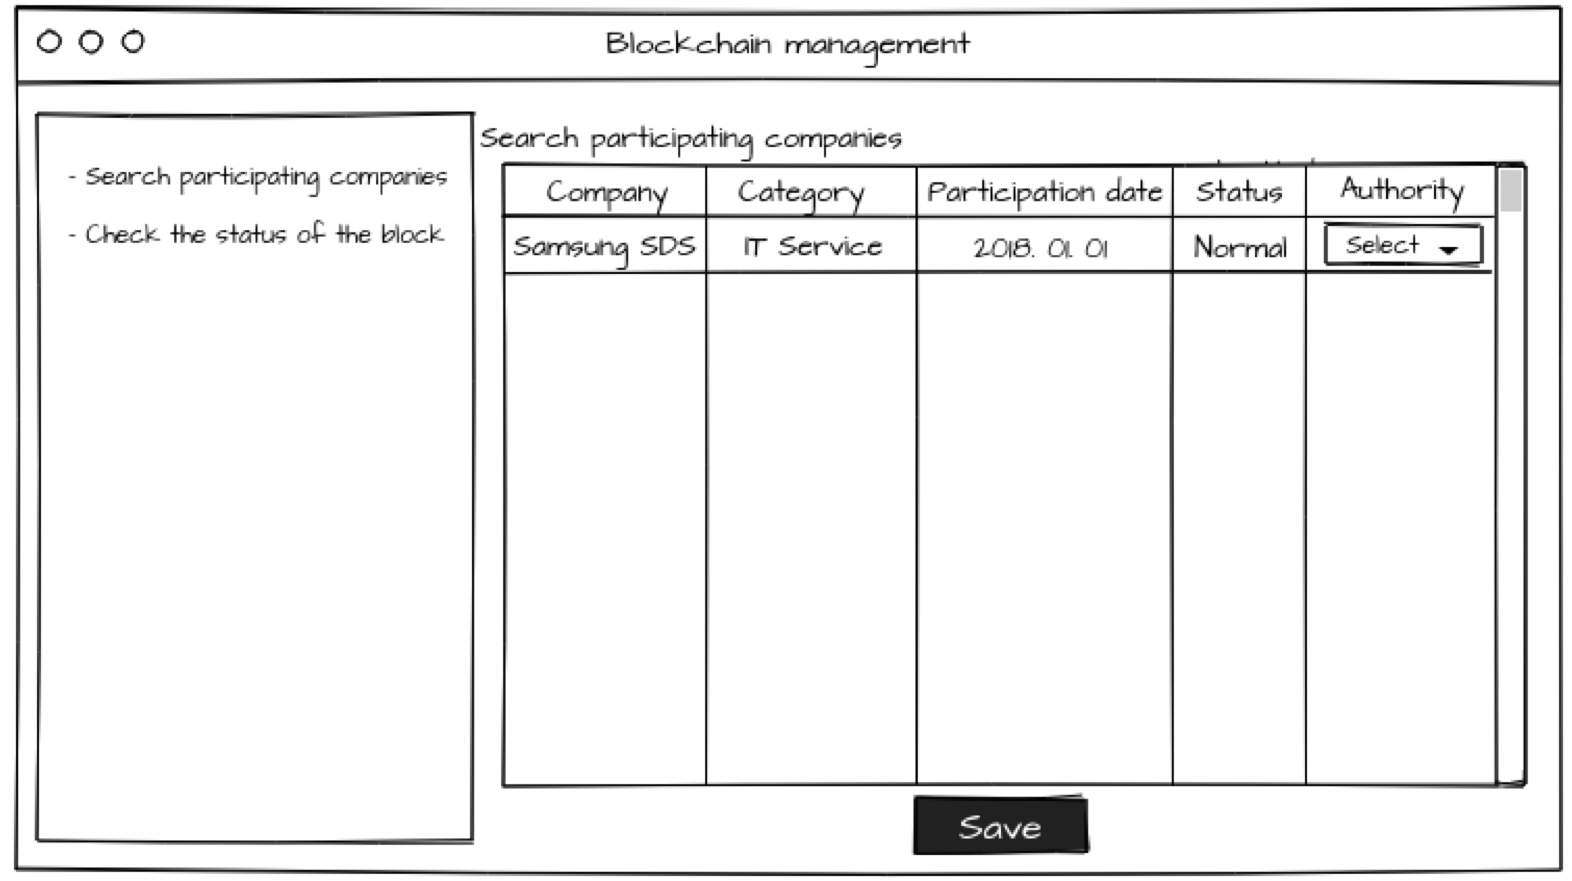
\includegraphics[width=89mm,scale=0.5]{school/blockchain_management.png}}
	\caption{Blockchain management search participating companies page for SDPS}
	\label{fig}
	\end{figure}
	
	Central execute of private block chain conduct process of discerning whether the company is trustworthy or not when trying to accept company to block chain as node, however, this process can be imperfect since it is done by person. Therefore, service for searching information of participated companies and supervising which company cheated on the chain is provided. The representative behavior of cheating is that some company reads transaction of data sent to the other company with access to sharing ledger. When central executes realizes this kind of cheating, they should make proper decision to handle the problem.\\
        \item \textit{Check the status of the block chain:} 
        \begin{figure}[htbp]
	\centerline{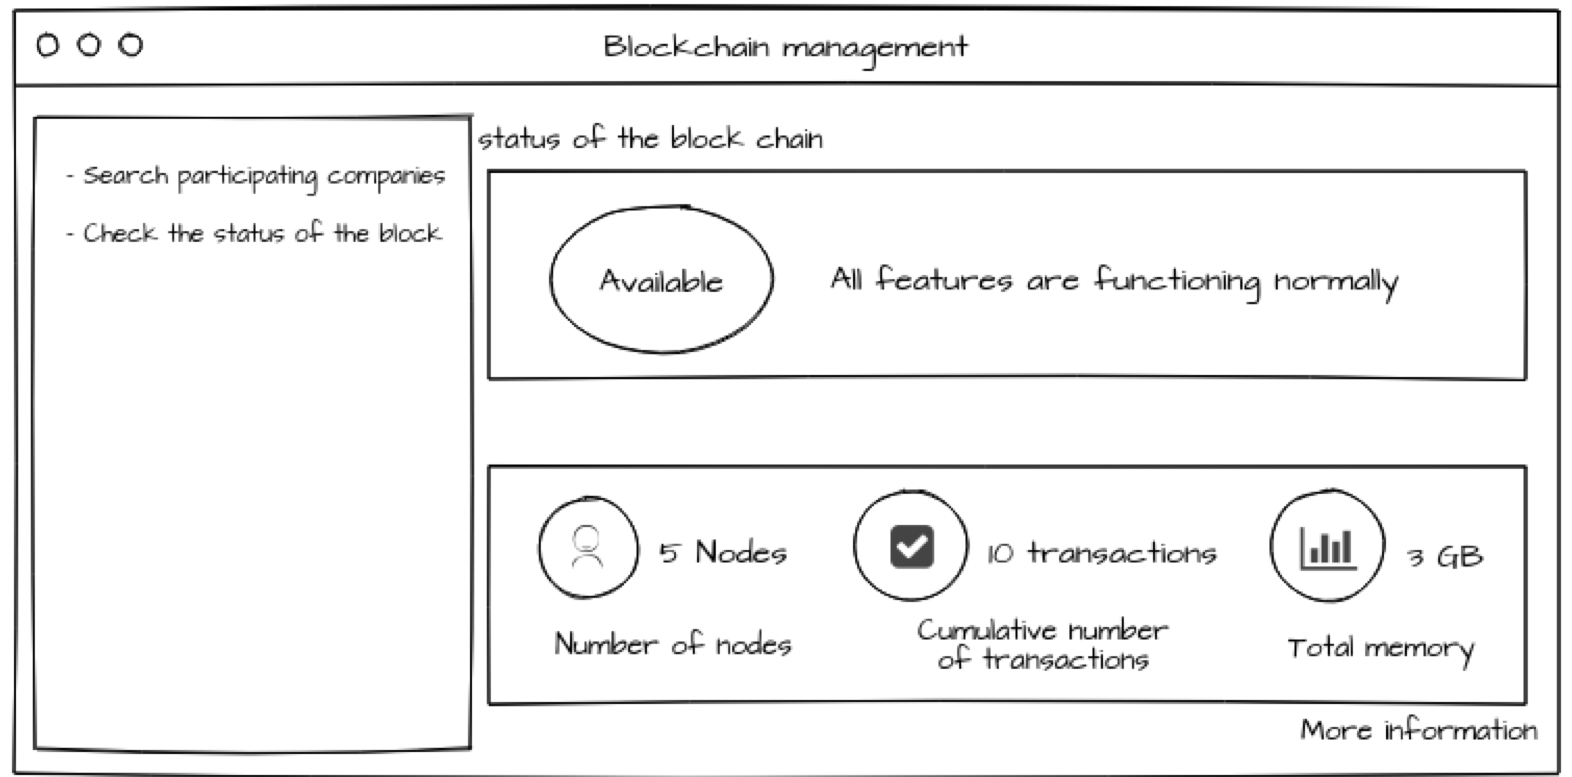
\includegraphics[width=89mm,scale=0.5]{school/blockchain_management2.png}}
	\caption{Blockchain management Check the status of the block chain page for SDPS}
	\label{fig}
	\end{figure}
        
        It conducts ‘health check’ function to the block chain periodically. If the block chain network falls into incapacity because of any errors, it marks ‘unavailable’. ‘Available’ mark is presented when there is no problem. With this function, state of the block chain network is recognized steadily so that we can deal with any kinds of errors rapidly.\\
    \end{enumerate}
\end{enumerate}

\subsection{Company}
Company members can remove unreliable and cumbersome certification which has high potential loss and cannot be assured regarding reliability from company’s recruitment process by using our application. Since the company is main target which takes data of certification through the block chain, it should be participated in the chain as node directly. Therefore, the company cannot but go through separate process of becoming member.\\
 \vspace{100mm}
\begin{enumerate}
	\item \textit {Registration page: }
	\begin{figure}[htbp]
	\centerline{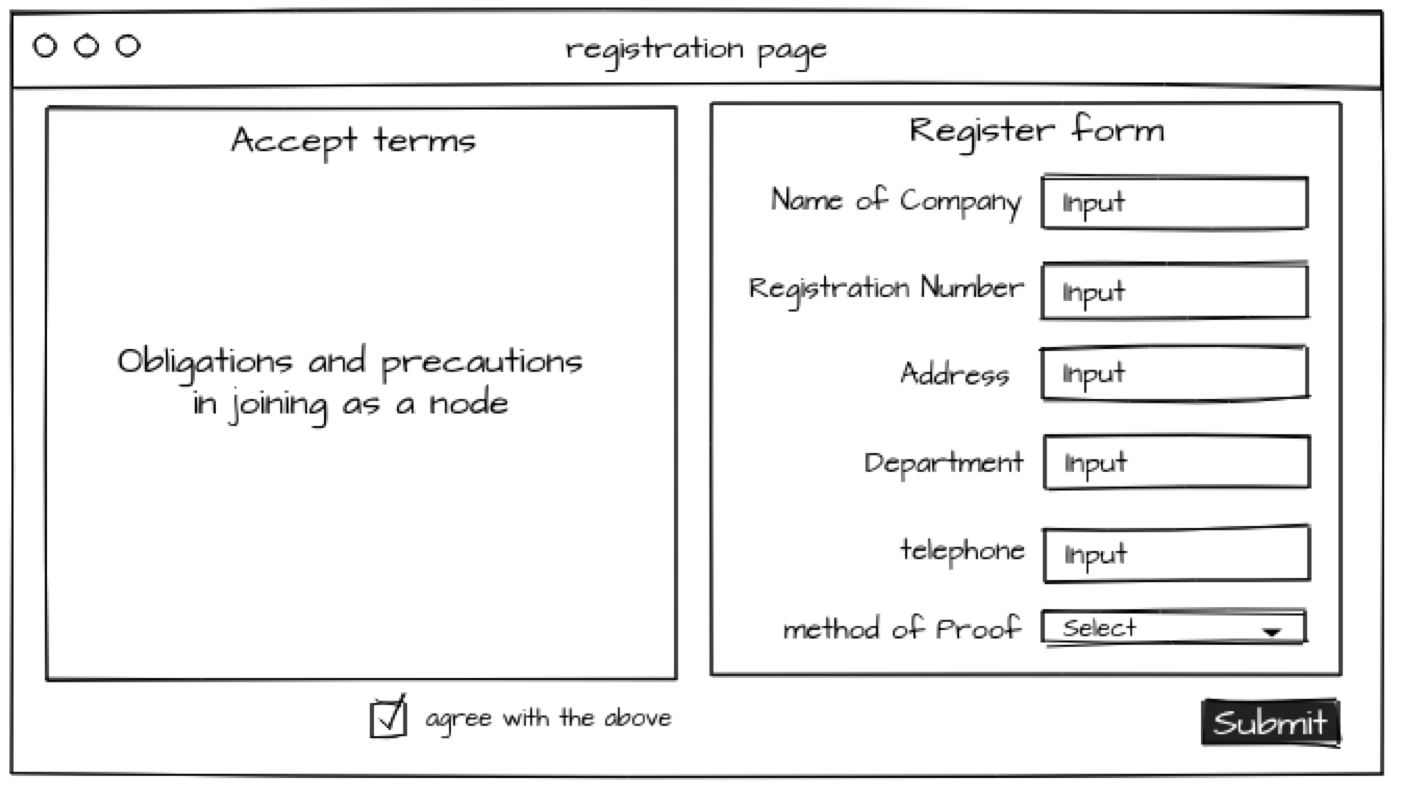
\includegraphics[width=89mm,scale=0.5]{company/register_page.png}}
	\caption{Registration page for SDPS}
	\label{fig}
	\end{figure}
	
	The company must insert id, password to use, detailed information of company, information of a person in charge of recruiting who takes data by using the block chain and trustworthy data from network’s central execute. Information in membership page entered by company’s person in charge of recruiting is transmitting to central executes’ page and administrator approves after identifying whether specific companies is so reliable that they could be joined in network as node or not. After approval, authority of participating in network as node is made. Node data of block chain is created by manager and the data is recorded based on input information from procedure of membership. Since the company is participated in block chain as node directly, distinct hash value is given to it, not like students. Other companies cannot identify the company based on the hash value, however, central execute can recognize each company which is mapped to the hash value. This can be applied as basic data for company monitoring.\\
    
    \item \textit {First Page (Log-in Page): }The company can login to web application with id and password. The login does not mean the direct access to block chain network. Instead, customer users can consume linked data through web application without any information about block chain at all. As we can see from this kind of view, our application service seems to exists to provide usability ultimately.\\
    \begin{enumerate}
    	\item  \textit {Log-in:} The company can access to web application linked with node data of block chain after central executes’ approval of node membership is made. The information of login is same with entered in membership page. \\
        \item  \textit {ID/PW search:} Since company’s person in charge of recruiting can be changed at any time, id and password which are used to get access to web application have possibility of being lost during process of transition. Therefore, our web application offers function of searching id and password of the company.\\
    \end{enumerate}
    
    \item \textit {Main page:} 
    \begin{figure}[htbp]
	\centerline{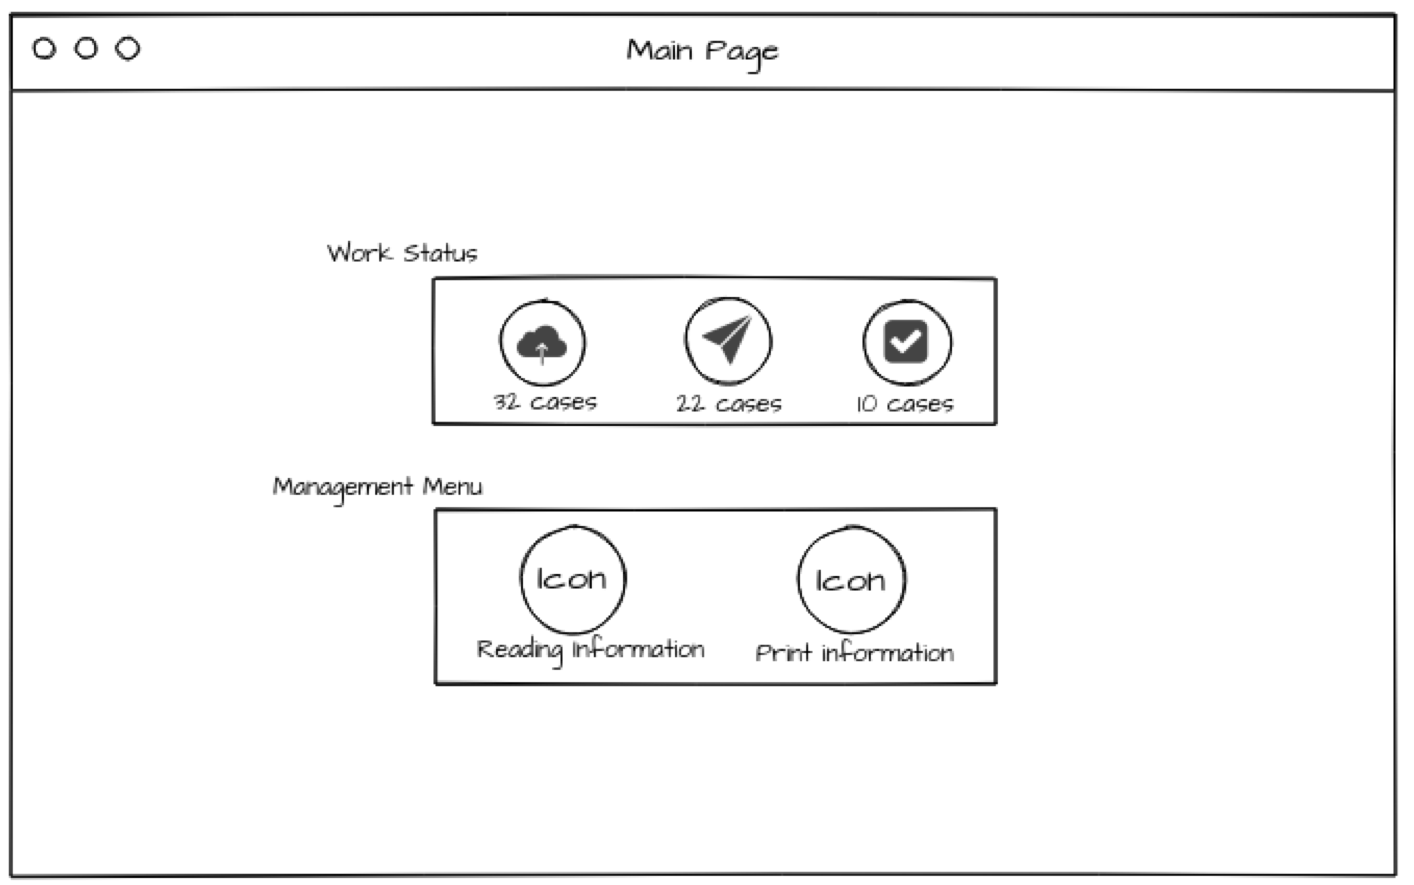
\includegraphics[width=89mm,scale=0.5]{company/mainPage.png}}
	\caption{Main page for SDPS}
	\label{fig}
	\end{figure}
   
    This is the first page presented after company member succeeded login. This page provides anchors of available menus and marks the numerical value of how many datasets of student information transmitted from central execute are there. Then, student information is listed chronologically.\\
    \begin{enumerate}
    	\item  \textit {Work state:} It marks the total number of received information of student presented in main page. Additionally, it lists a few student information chronologically and provides function of anchor by enabling users to move on to page where they can check the data when the information is clicked.\\
        \item  \textit {Management menu:} Lists functions which can be conducted by company members and offers navigation towards those functions.\\
    \end{enumerate}
    
       \item \textit {Reading information page:} The purpose of using the application by company members is to receive and read student information needed for process of recruiting. Thus, transmitted student data through block chain can be listed, read and even printed if needed.\\
       
     \vspace{70mm}  
    \begin{enumerate}
    	\item   \textit {Reading information:} 
	 \begin{figure}[htbp]
	\centerline{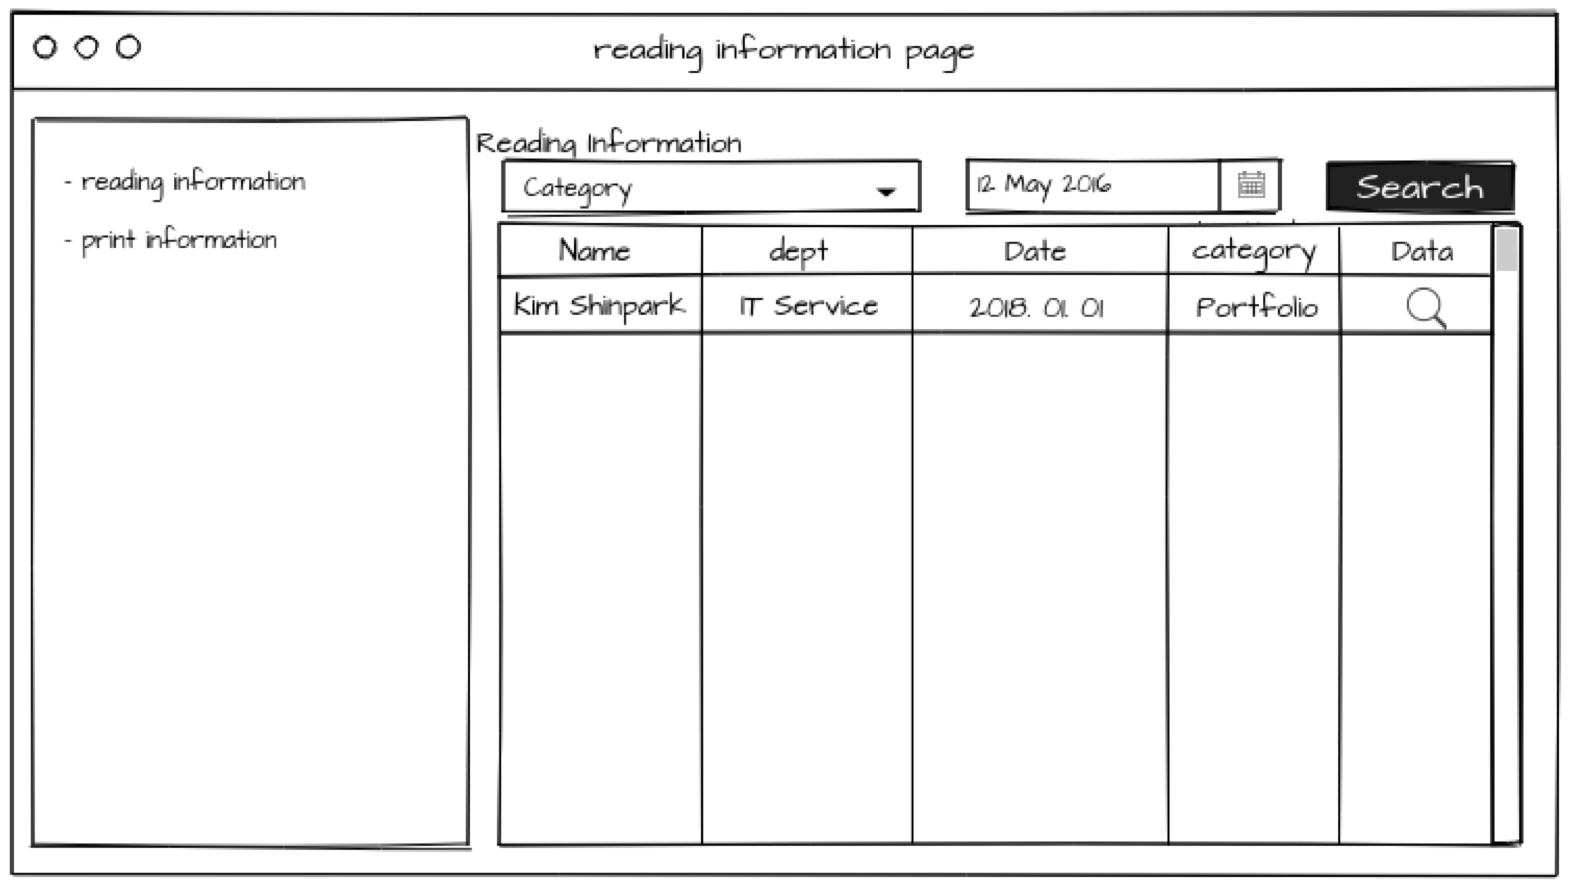
\includegraphics[width=89mm,scale=0.5]{company/func1.png}}
	\caption{Main page for SDPS}
	\label{fig}
	\end{figure}
	
	Information received through block chain of students who applied for specific company is listed on the page and presented with table form. Specific information of the student can be read if each row of presented table is clicked.\\
        \item  \textit {Print information:} 
         \begin{figure}[htbp]
	\centerline{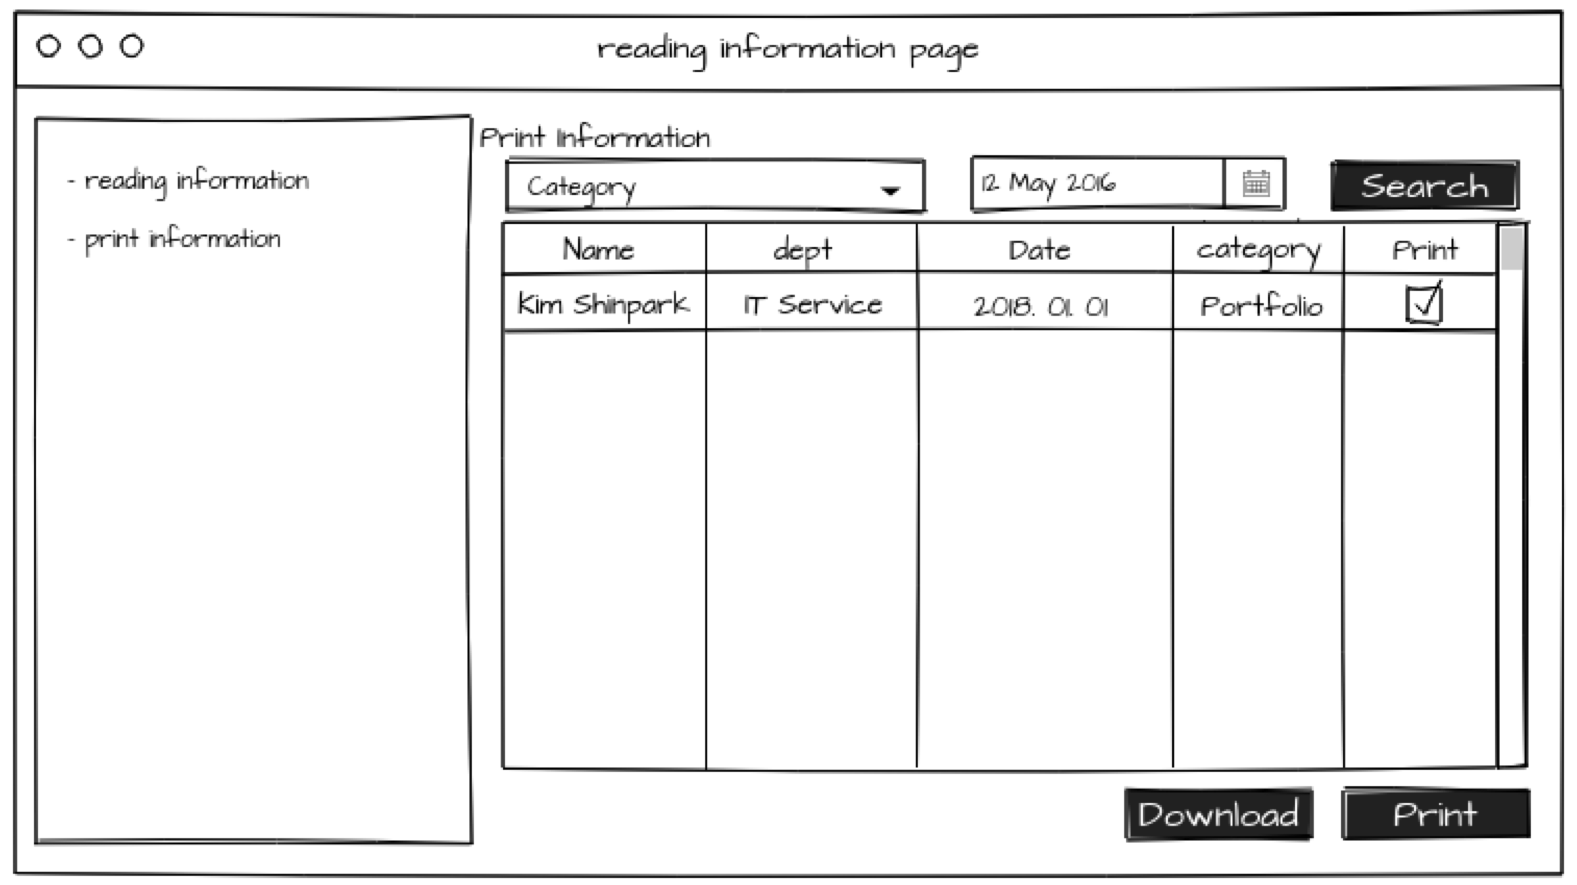
\includegraphics[width=89mm,scale=0.5]{company/func2.png}}
	\caption{Main page for SDPS}
	\label{fig}
	\end{figure}
        
        There might be situations that company should keep applicant related information as paper inevitably during recruiting process. Therefore, our application provides function enabling company to print students’ data received through private block chain.\\
    \end{enumerate}
        
\end{enumerate}


\end{document}
